\documentclass[10pt, conference, letterpaper]{IEEEtran}
\IEEEoverridecommandlockouts
% The preceding line is only needed to identify funding in the first footnote. If that is unneeded, please comment it out.
\usepackage[table]{xcolor}
\usepackage{enumitem}
\usepackage{setspace}
\usepackage{booktabs}
\usepackage{graphicx}
\usepackage{subcaption}
\usepackage{listings}
\usepackage{pgfplots}
\pgfplotsset{compat=1.16}
\usepackage{pgfplotstable}
\usepackage{tikz}
\usetikzlibrary{patterns}
\usepackage[justification=centering]{caption}
\usepackage{url}
\usepackage{tabularx}
\usepackage{booktabs}
\usepackage{multirow}

\usepackage{listings}
\usepackage{xcolor}
\usepackage{caption}

\definecolor{codebg}{RGB}{245,245,245}
\definecolor{codeborder}{RGB}{210,210,210}

\lstdefinestyle{ndnsfstyle}{
    backgroundcolor=\color{codebg},
    basicstyle=\ttfamily\footnotesize,
    frame=single,
    rulecolor=\color{codeborder},
    columns=fullflexible,
    breaklines=true,
    showstringspaces=false,
    xleftmargin=6pt,
    xrightmargin=6pt,
    framexleftmargin=6pt,
    framexrightmargin=6pt,
    framesep=4pt,
    aboveskip=4pt,
    belowskip=2pt,
    captionpos=b
}

\renewcommand{\lstlistingname}{API}
% correct bad hyphenation here
\hyphenation{net-works}


% --- code/spec block ---
\usepackage{listings}
\usepackage{tcolorbox}
\tcbuselibrary{listings,skins,breakable}

\newtcblisting{proto}{
  listing only,
  breakable,                 % 允许跨页
  colback=white,             % 背景
  colframe=black!60,         % 边框颜色
  boxrule=0.5pt,             % 边框粗细
  arc=2pt,                   % 圆角
  left=6pt,right=6pt,
  top=6pt,bottom=6pt,
  listing options={
    basicstyle=\ttfamily\small, % 等宽字体 + 字号
    breaklines=true,            % 自动换行
    columns=fullflexible,       % 字符对齐更像等宽
    keepspaces=true,            % 保留空格（缩进关键！）
    showstringspaces=false
  }
}


\begin{document}

%
% paper title
% Titles are generally capitalized except for words such as a, an, and, as,
% at, but, by, for, in, nor, of, on, or, the, to and up, which are usually
% not capitalized unless they are the first or last word of the title.
% Linebreaks \\ can be used within to get better formatting as desired.
% Do not put math or special symbols in the title.
\title{NDNSF: A Framework for Secure and Reliable Service-Oriented Applications over NDN}
%
%
% author names and IEEE memberships
% note positions of commas and nonbreaking spaces ( ~ ) LaTeX will not break
% a structure at a ~ so this keeps an author's name from being broken across
% two lines.
% use \thanks{} to gain access to the first footnote area
% a separate \thanks must be used for each paragraph as LaTeX2e's \thanks
% was not built to handle multiple paragraphs
%

%LW: remove for submission for anonymity
%\author{
%Tianxing Ma, Eddie Jacobs, Lan Wang\\
%University of Memphis \\
%\{tma1, eljacobs, lanwang\}@memphis.edu
%}

\maketitle

\pagestyle{plain}

% As a general rule, do not put math, special symbols or citations
% in the abstract or keywords.
\begin{abstract}
Distributed service-oriented applications require secure discovery, provider selection, and access control under changing resource availability. Earlier service information may not reflect a provider's suitability for a particular request. We present NDNSF, a distributed, data-driven service framework built on Named Data Networking (NDN). Its basic invocation workflow uses Request, acknowledgment (ACK), Selection, and Response Data to solicit provider participation, select executors from their feedback, and deliver results. NDNSF uses a data synchronization protocol to disseminate these messages. Provider feedback and customizable selection allow users to choose executors according to task requirements and current resource availability. To protect task requirements disclosed during discovery, NDNSF uses name-based access control with attribute-based encryption (NAC-ABE). This allows multiple authorized providers to assess a request while keeping its discovery descriptor confidential from readers lacking the required decryption capability, without enumerating provider identities. Under one ABE authority and the same set of public parameters, NDNSF also aggregates service permissions in one decryption key per entity. Separating service permissions from signing identity supports credential reuse across compatible services and applications, with baseline trust rules focused on signing authority rather than service-permission lists. We analyze credential counts and identify policy-dependent distribution and update costs, then evaluate invocation behavior against NDN Service Call (NSC) and gRPC in wired and wireless experiments. In our single-provider wired experiments with packet loss, NDNSF achieves higher completion rates than NSC and rates comparable to gRPC. With multiple intermittently available providers, it achieves higher completion rates than the fixed-provider baselines by dynamically selecting available providers.
 

\end{abstract}

% Note that keywords are not normally used for peerreview papers.
\begin{IEEEkeywords}
Information Centric Networking, Named Data Networking, Secure Service Framework, NDN Synchronization
\end{IEEEkeywords}

\section{Introduction}
Distributed service-oriented applications~\cite{channabasavaiah2003migrating} power everything from global cloud infrastructure to real-time industrial automation.  They operate over networks of computers where services are the primary abstraction. For example, in edge AI systems, WiFi and cellular base stations may provide storage and AI inference/training services to end devices, while also offloading compute-intensive tasks to cloud services. As another example, a UAV network may adopt a service-oriented design to coordinate a ground station and multiple drones: each drone exposes flight-control services invoked by the ground station, while drones may also request services from one another (e.g., for sensing or data processing).  Service frameworks provide the software infrastructure to develop, deploy, and manage such applications.  

NDNSF is motivated by applications in which provider availability and task suitability change over time. A UAV's position and sensing conditions may change, while an inference provider's workload and available memory may vary. Earlier service information describes an offered capability, but may not indicate whether the provider can serve a particular request at that moment. Applications therefore need request-specific participation feedback before selecting executors. NDNSF connects this feedback to user selection and subsequent execution; feedback is not a resource reservation and may become outdated before execution.

In today’s Internet, gRPC~\cite{grpc} is widely used for high-performance remote procedure calls, REST~\cite{fielding2000architectural} supports stateless HTTP-based interactions, and message-queue systems~\cite{john2017mqsurvey} enable asynchronous decoupled communication. Despite their widespread adoption, particular deployments of these frameworks can face limitations in dynamic and large-scale environments. \emph{Scalability} can be constrained when provider selection requires repeated point-to-point exchanges. \emph{Reliability} can be impacted by endpoint binding and load concentration, which create performance bottlenecks and potential single points of failure. \emph{Security} based only on channels protects data in transit; object-level confidentiality requires additional encryption.
% since IP does not natively bind security to named content or enforce fine-grained access control over data objects.

Named Data Networking (NDN)~\cite{zhang2014named} provides an alternative, data-centric networking model in which communication is driven by named data rather than host addresses. Consumers issue Interests to retrieve Data packets, and each Data packet is cryptographically signed to ensure integrity and authenticity, with optional encryption for confidentiality. NDN improves \emph{scalability} through in-network caching and native multicast delivery, allowing multiple consumers to retrieve the same published Data. It enhances \emph{reliability} by decoupling communication from fixed endpoints, enabling retrieval from caches or alternative sources under failures or mobility. Signatures validated under appropriate trust rules support authenticity and integrity; encryption is additionally needed to restrict content access. These properties make NDN a strong foundation for secure service-oriented applications.

\emph{Despite the above advantages, building service-oriented applications over NDN remains challenging because applications must coordinate discovery, access control, and invocation.} To address this gap, we design the Named Data Networking Service Framework (NDNSF), a modular framework for building secure and distributed service-oriented applications with minimal NDN-specific complexity. NDNSF provides three core capabilities: (i) \textbf{service publication and secure discovery}, (ii) \textbf{fine-grained, name-based access control using attribute-based encryption}, and (iii) \textbf{service invocation with dynamic provider selection}. In particular, NDNSF introduces a \textbf{one-to-many service model with customizable provider-selection strategies}, enabling applications to choose providers based on runtime metrics such as computational capacity, queue state, and network delay.

Providers assess task requirements against their current resources and return positive ACKs when willing to participate. The user then applies a customizable selection strategy to choose among these candidates.

We evaluate NDNSF against NDN Service Call (NSC)~\cite{meirovitch2021nsc} and gRPC. In our single-provider wired experiments with packet loss, NDNSF achieves higher completion rates than NSC and rates comparable to gRPC. In scenarios with multiple heterogeneous and intermittently unavailable providers in both wired and wireless networks, NDNSF achieves higher success rates in the evaluated configurations by selecting among available providers, whereas the configured baselines use a fixed provider. We also evaluate selective acknowledgment under provider overload and user-defined provider-selection strategies.

NDNSF's basic service invocation workflow is driven by four Data types and combines protected request dissemination, provider participation feedback, user selection, and execution. Its authorization design has three aspects:
\begin{enumerate}
\item \textbf{Confidential One-to-Many Service Discovery.} NAC-ABE encrypts discovery descriptors containing task requirements that providers need to decide whether to participate, without requiring the requester to list provider identities. 
\item \textbf{Aggregated Service Credentials.} Under one ABE authority and the same set of public parameters, each entity can hold one decryption key (DKEY) encoding multiple service permissions. Section~\ref{sec:credential-cost} separates credential counts from distribution and update costs.
\item \textbf{Reusable Identity Credentials with Simple Trust Rules.} ABE policies represent service permissions, so baseline trust rules can focus on which identities and keys may sign messages rather than listing each entity's service permissions. Identity-signing credentials remain reusable across applications sharing the same trust configuration.
\end{enumerate}
These features use the access-control capabilities of NAC-ABE~\cite{zhang2018nac,dulal2023nac-abe}. Permission aggregation is inherited from ABE; we analyze its organization for service permissions.
 

\section{BACKGROUND}
\label{sec:background}
NDN~\cite{zhang2014named,afanasyev2018brief} shifts networking from a host-centric to a data-centric communication model.  In this section, we briefly review NDN and two NDN-based mechanisms used by NDNSF.

\subsection{NDN in a Nutshell}

\begin{figure}[]
    \centering
    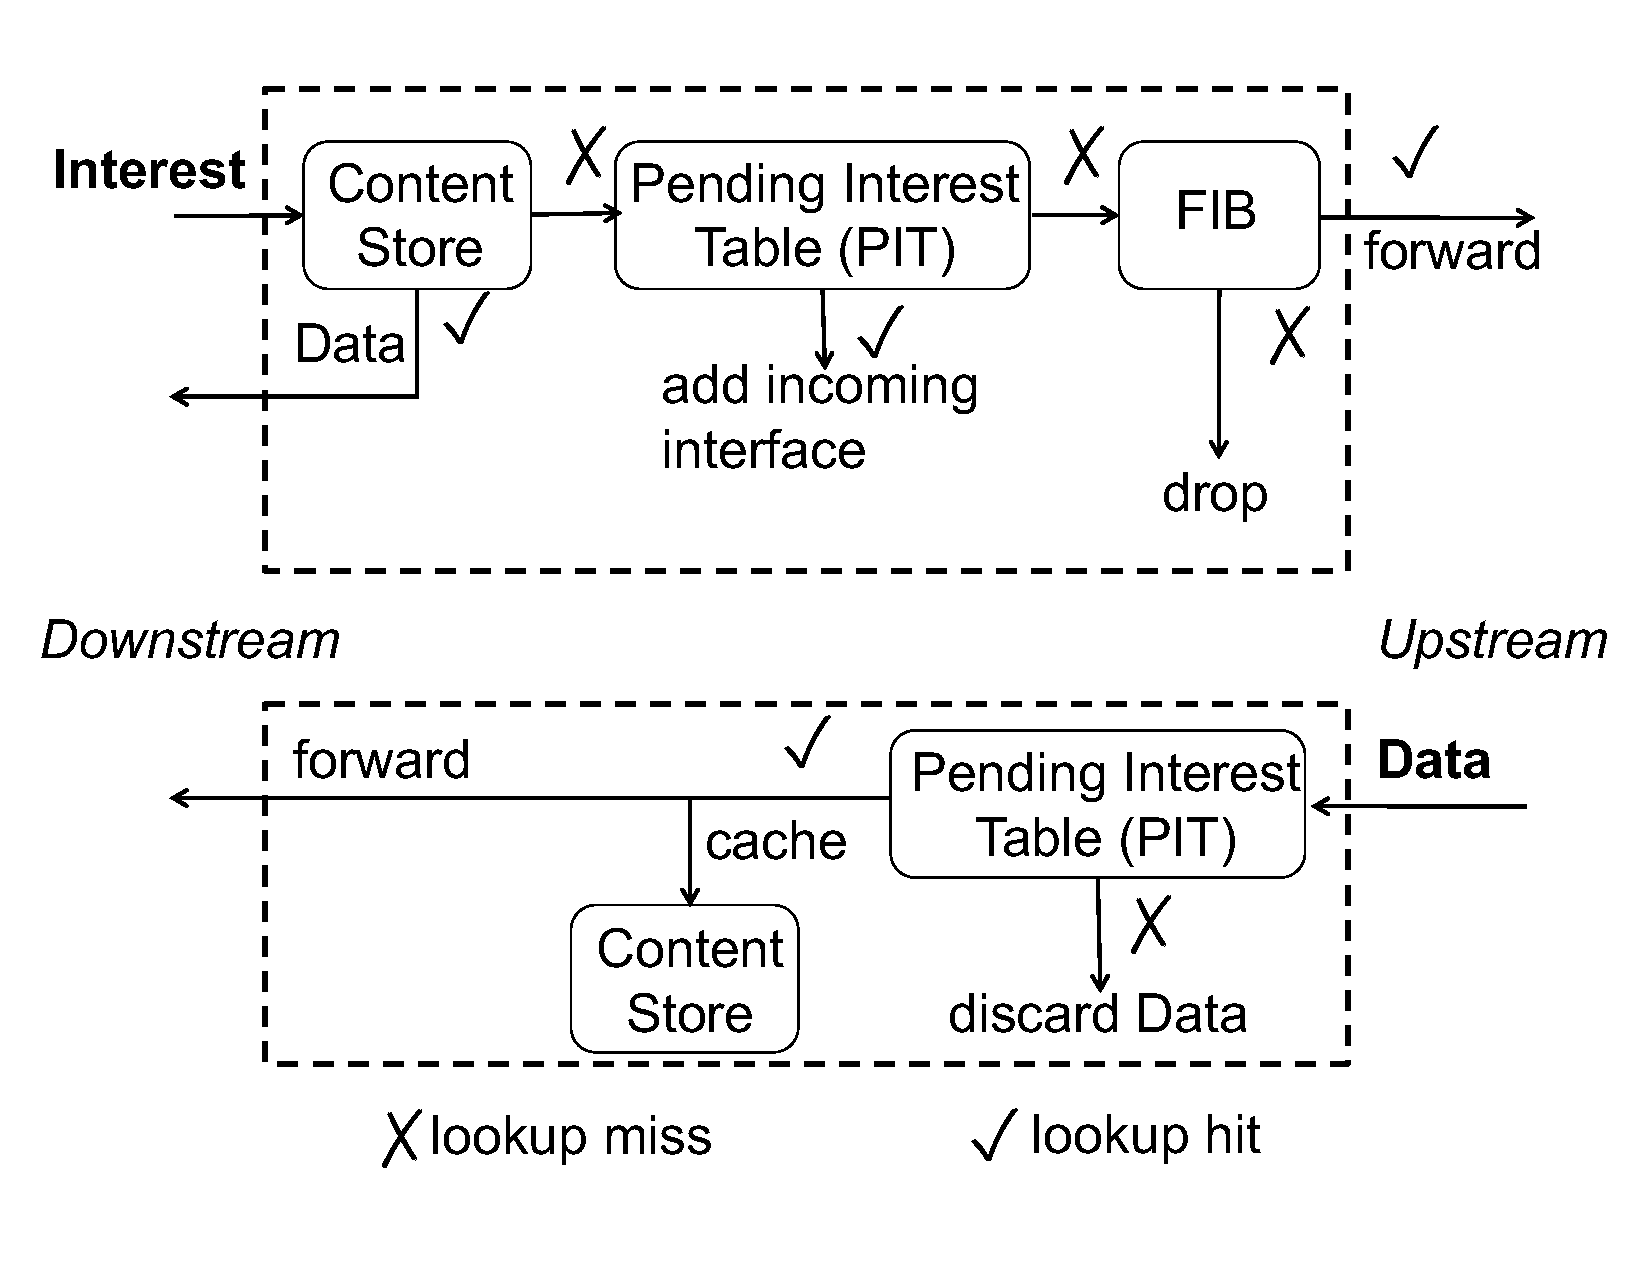
\includegraphics[width=.9\columnwidth]{figures/ndn-forwarder.pdf}
    \vspace{-3mm}
    \caption{NDN Forwarding Process (adapted from~\cite{afanasyev2018brief}, Fig.~3)}
    \label{fig:ndn-forwarder}
    \vspace{-3mm}
\end{figure}

NDN employs a receiver-driven request-response model based on two packet types: \textit{Interest} and \textit{Data}. A consumer sends an Interest packet specifying the desired data name, and the network forwards the Interest toward potential data sources using the data name, including producers and in-network caches. Once a matching Data packet is located, it is returned along the reverse path established by the Interest.

To support this process, each NDN forwarder maintains three data structures: Forwarding Information Base (FIB), Pending Interest Table (PIT), and Content Store (CS). The FIB stores name-prefix routes used by the forwarding strategy, the PIT tracks pending Interests and can aggregate compatible Interests so that a matching Data packet can satisfy multiple consumers, thereby enabling multicast delivery, and the CS caches Data packets for future requests, which can reduce retrieval latency and bandwidth consumption. Figure~\ref{fig:ndn-forwarder} illustrates how these structures operate during Interest and Data forwarding. By decoupling data from network locations and maintaining PIT state, NDN naturally enables in-network caching, multicast data delivery, and adaptive forwarding~\cite{yi2013case}.  It can also support content delivery networks (CDNs), mobile ad-hoc networking (MANET), and delay-tolerant networking (DTN)~\cite{afanasyev2018brief}.

NDN also adopts a data-centric security model in which each Data packet carries a signature. A producer's cryptographic signature, validated under trust-schema rules specifying authorized signing keys~\cite{yu2015trust}, enables consumers to verify data authenticity and integrity independently of the communication path or retrieval source, which is particularly advantageous in environments with caching and replicated content.

\subsection{NDN Sync}

In a multi-party distributed NDN application, the participants need to learn the names of data newly produced by others, so that they can retrieve new data promptly.  This functionality is provided by Distributed Dataset Synchronization, or Sync in short (\cite{li2018brief,moll2022sok}). Instead of relying on a central node, Sync participants exchange summaries of their data names and discover differences (i.e., new data names). A number of NDN Sync protocols have been developed over the last decade, such as ChronoSync~\cite{zhu2013let}, PSync~\cite{zhang2017scalable}, and State Vector Sync (SVS)~\cite{moll2021svs}. NDNSF builds on Sync to announce service-message publications without centralized coordination. In particular, we use the NDN-SVS implementation~\cite{ndnsvs-github}.

%\subsection{NDN Service Discovery (NDNSD)}
%TODO: add more details (those relevant to our paper) about how NDNSD works 
% Service discovery is crucial for modern distributed applications, and NDNSD \cite{dulal2022ndnsd} addresses this by offering a fully distributed and scalable service discovery protocol for NDN, utilizing NDN's data synchronization capabilities for efficient service publishing and discovery without external infrastructure dependencies.

\subsection{NAC-ABE}

\begin{figure}[]
    \centering
    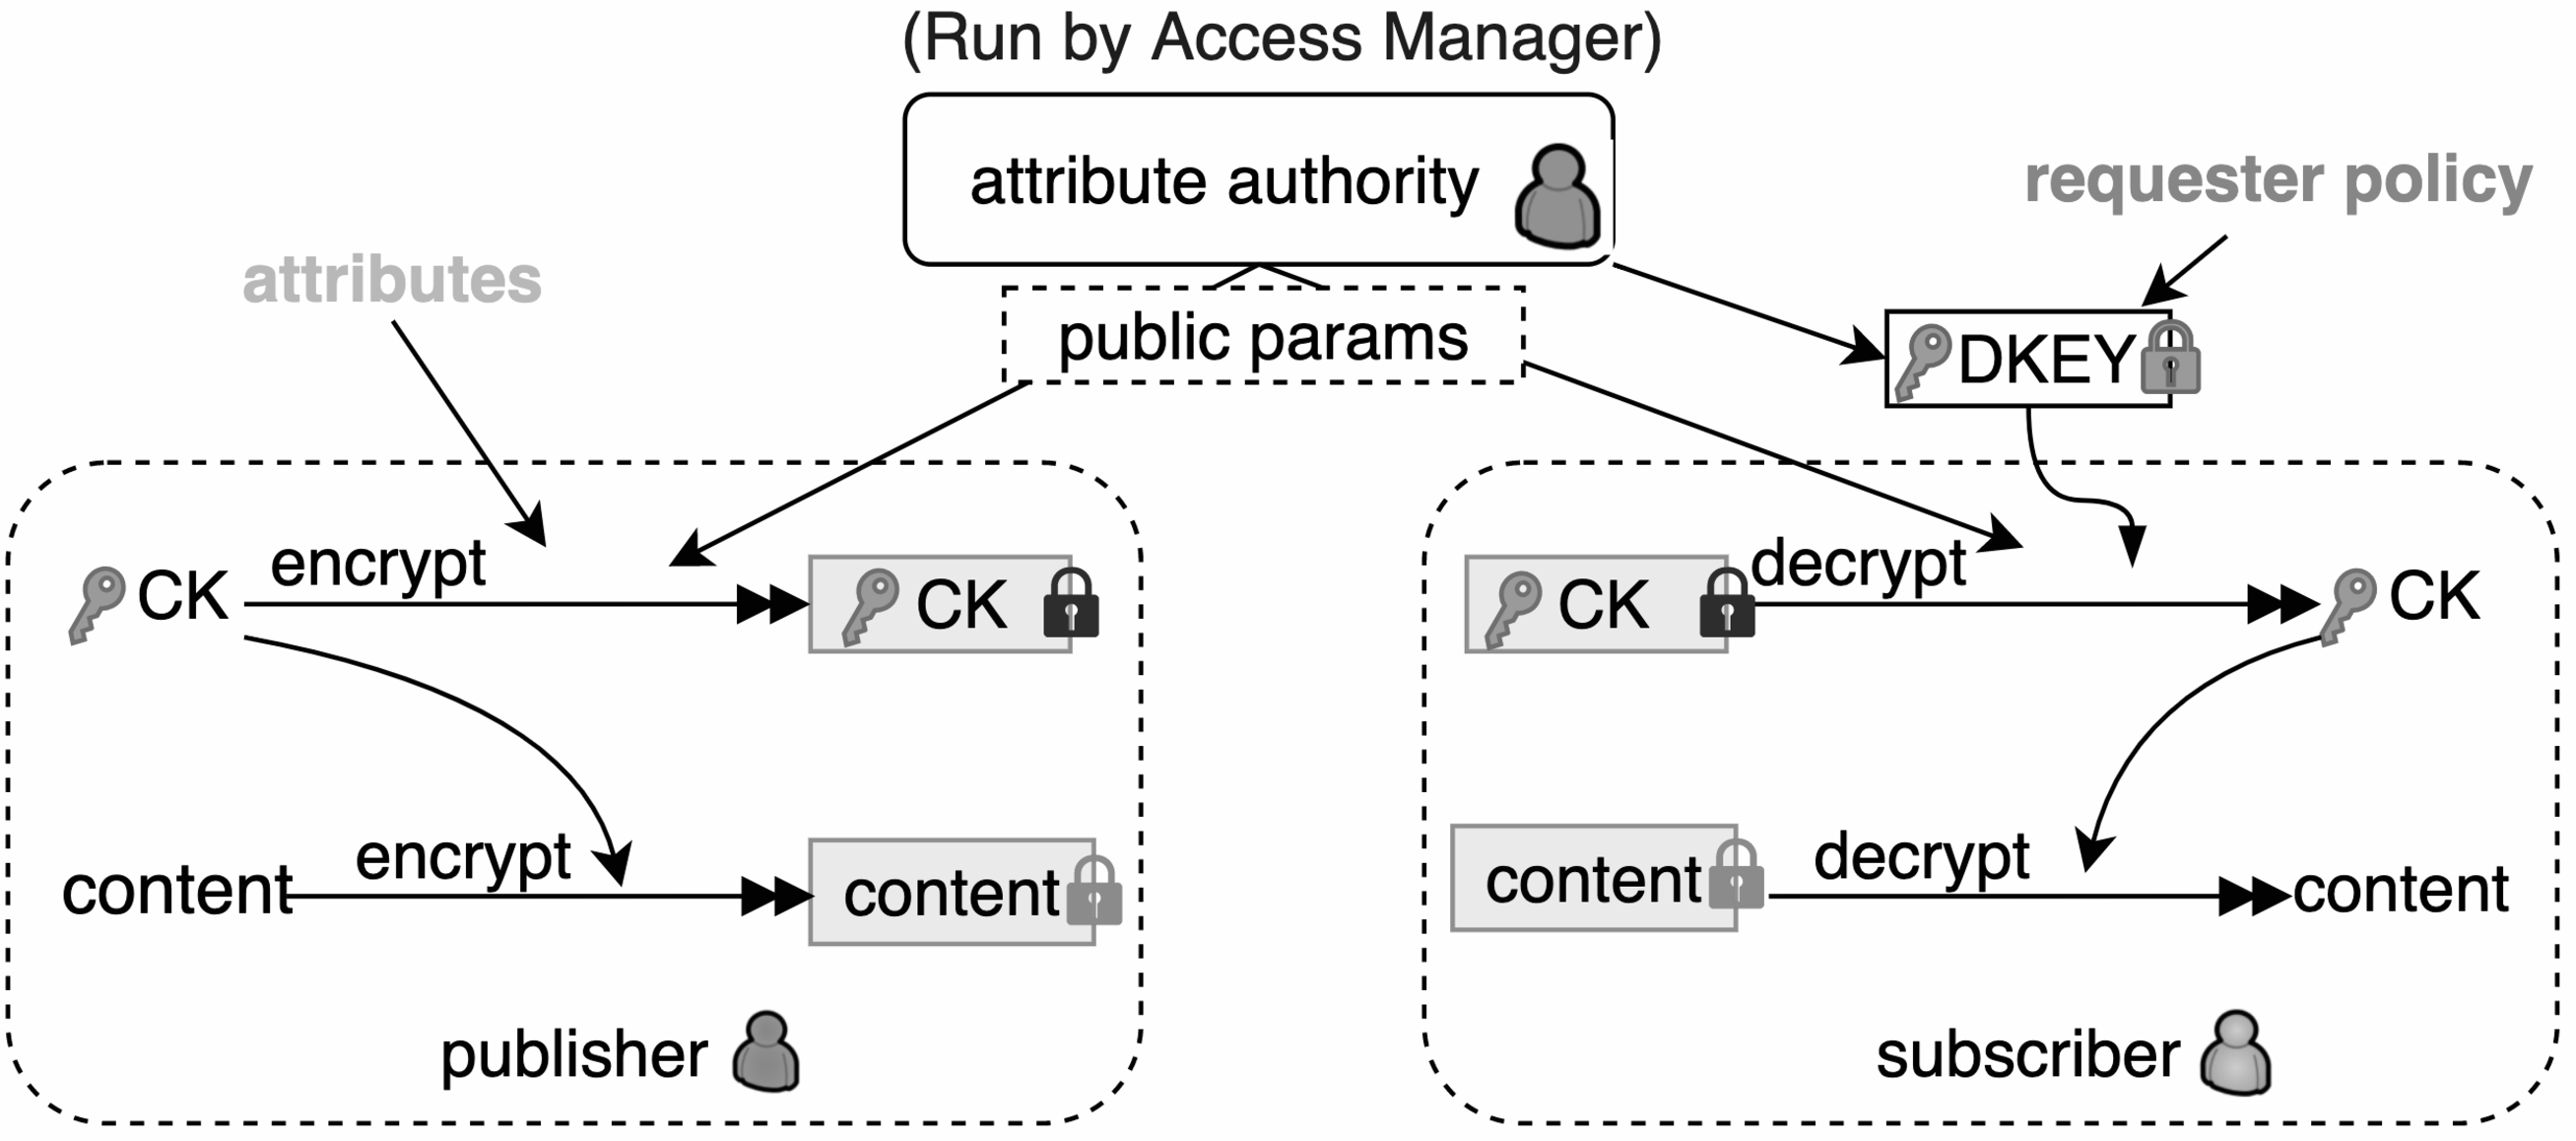
\includegraphics[width=.9\columnwidth]{figures/kp-abe-scheme.pdf}
    \caption{Encryption and Decryption with KP-ABE~\cite{dulal2023nac-abe}}
    \label{fig:kp-abe}
    \vspace{-3mm}
\end{figure}

NAC automates access-key distribution for named Data~\cite{zhang2018nac}. NDNSF leverages NAC-ABE~\cite{dulal2023nac-abe} to provide fine-grained access control and automated key management.
More specifically, we use Key-Policy Attribute-Based Encryption (KP-ABE)~\cite{goyal2006attribute} provided by NAC-ABE, where data is encrypted under a set of attributes, and each user’s decryption key (DKEY) encodes an access policy over those attributes.

In NAC-ABE, an Attribute Authority manages system attributes and issues decryption keys for access control (Figure~\ref{fig:kp-abe}). During initialization, it generates public parameters and a master secret key. The public parameters are distributed to all participants for use in cryptographic operations, while the master key is kept by the Attribute Authority to generate user-specific decryption keys (DKEYs) according to their authorized access policies.  Each data object is encrypted using a symmetric Content Key (CK), and the CK is then encrypted using ABE under the data object’s associated attributes. When retrieving data, a participant first obtains the encrypted CK (whose name is included in the data object), then decrypts it using their DKEY. The recovered CK is subsequently used to decrypt the data object itself. This hybrid design improves efficiency by applying expensive ABE operations only to the small CK, while using fast symmetric encryption for the bulk data. DKEY size can grow with policy complexity and may require segmentation~\cite{dulal2023nac-abe}.

%Each DKEY is encrypted using the corresponding participant's public key. The encrypted DKEY is packaged into an NDN data object and named according to specific conventions. Each participant retrieves the appropriate encrypted DKEY packet using these naming conventions and decrypts it with their private key to obtain their DKEY.


%\subsubsection{Bloom Filter}
%A Bloom filter \cite{lu2005bloom} is a probabilistic data structure, and it efficiently represents a set of elements and allows for fast membership queries with minimal space requirements. While it may occasionally produce false positives, it never produces false negatives, making it suitable for applications where false positives are acceptable but false negatives are not.

%\subsubsection{Protocol Buffers}
%Protocol Buffers (protobuf) \cite{protobuf_dev} is a language-neutral and platform-neutral method to serialize structured data, offering a simple and efficient way to define data formats. With protobuf, developers can define the structure of their data using a simple interface definition language and generate code in various programming languages to serialize and deserialize data in a compact and efficient binary format.
 

\section{DESIGN}
\begin{figure*}[t]
    \centering
    \begin{tikzpicture}
      \node[inner sep=0pt, anchor=south west] (uav) at (0,0)
        {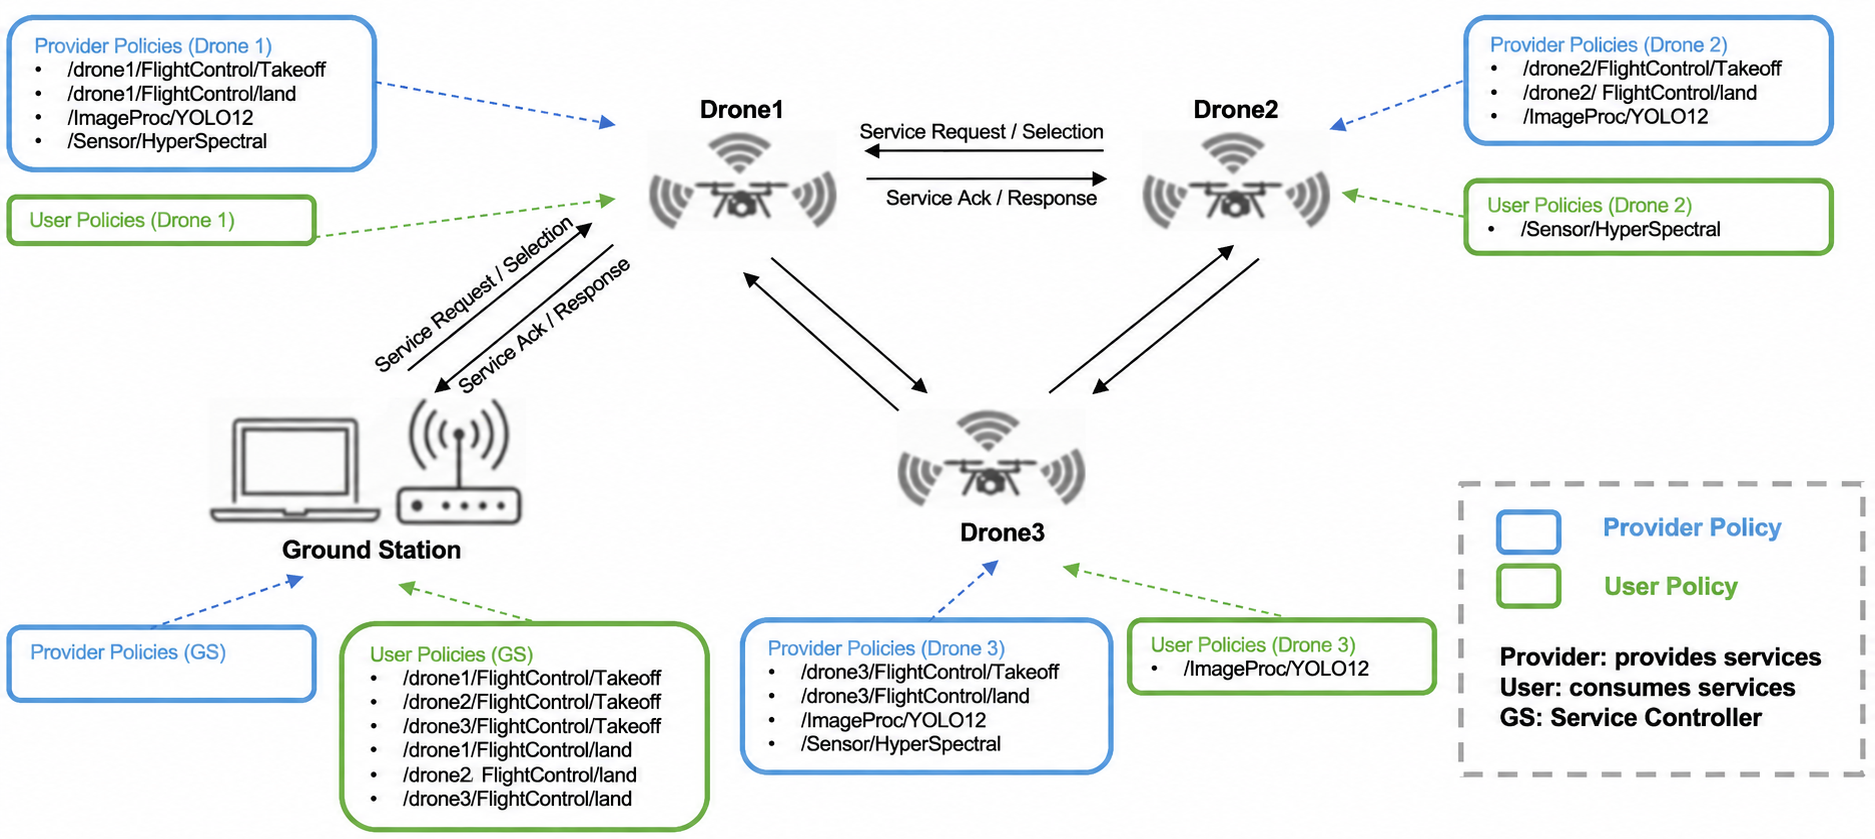
\includegraphics[width=.8\textwidth]{figures/drones-corrected.png}};
      \node[anchor=west, fill=white, inner sep=0pt,
        font=\sffamily\fontsize{5.2pt}{6pt}\selectfont]
        at ([xshift=.17\textwidth,yshift=14pt]uav.south west)
        {/drone2/FlightControl/land};
    \end{tikzpicture}
    \caption{UAV Network Application Example}
    \vspace{-3mm}
    \label{fig:UAV-NDNSF}
\end{figure*}

An NDN service framework should provide three core functions: (1) \textbf{service publication and discovery} mechanisms that enable providers to publish services and users to locate available services; (2) \textbf{access control mechanisms}, including authorization and enforcement, that regulate which entities may provide or access services; and (3) \textbf{service invocation mechanisms} that allow users to request services.

NDNSF combines \textbf{\emph{fine-grained access control}} and \textbf{\emph{dynamic provider selection}} in a \textbf{\emph{one-to-many service model}}. It uses NAC-ABE to control which entities may provide or access services. Under one ABE authority, an entity's service permissions can be encoded in a single decryption key (Section~\ref{sec:service-controller}). In the four-message invocation flow, authorized providers return ACKs indicating their willingness to execute the current task, optionally including resource information. The user combines this feedback with application-specific criteria to select one or more providers (Section~\ref{sec:provider-selection}). The user then shares the input decryption key only with the selected providers (Section~\ref{sec:messages}). Participation feedback thus guides provider selection, which determines access to the protected task input.
% (3) \textbf{security mechanisms} that ensure the integrity, authenticity, and confidentiality of service messages; and  
% and illustrate how our design choices support the following design goals:
%(a) \emph{Generality}: support diverse service types and adapt to varying application requirements;
%(b) \emph{Reliability}: tolerate failures and maintain service availability under adverse network conditions; and
%(c) \emph{Scalability}: accommodate new users and providers without complex configuration and significant performance degradation.

%\subsection{Design Assumptions}

%Given the distributed nature of the proposed service framework, we assume that candidate service providers are reachable at the network layer when service interactions are initiated. This assumption is consistent with prior NDN-based service designs and does not preclude temporary disconnections caused by mobility or network dynamics.

%In addition, as with all NDN applications, NDNSF assumes that participating entities have completed the standard NDN bootstrapping process. Specifically, each entity is expected to possess the necessary trust anchors, certificates, and trust schemas required to enable data-centric security and name-based trust verification.


\subsection{Design Overview}

In an NDNSF-based distributed application, \emph{Service Providers} process requests and generate responses, \emph{Service Users} issue requests and consume responses, and the \emph{Service Controller} authorizes providers and users and defines their service permissions.  Figure~\ref{fig:UAV-NDNSF} illustrates these interactions in a UAV network. Drones act as \emph{Service Providers} offering flight-control and peer services (e.g., image processing or sensing), while the ground station serves as a \emph{Service User}. The \emph{Service Controller} may reside on the ground station or a dedicated in-network server.

%To support the functionalities of these entities, NDNSF consists of four core functional modules:
%(1) \textbf{Service Provider Bootstrap}, which enables Service Providers to obtain from the Service Controller the services they are authorized to offer and the necessary NAC-ABE keys; 
%(2) \textbf{Service User Bootstrap}, which enables Service Users to obtain from the Service Controller the services they are authorized to access and the necessary NAC-ABE keys;
%(3) \textbf{Secure Service Communication}, which ensures authenticity, integrity, and confidentiality of service messages over NDN; and
%(4) \textbf{Provider Selection}, which manages interactions among multiple Service Providers using different selection strategies.

\subsection{Service Publication and Discovery}

NDNSF discovers candidate providers through the Request--ACK exchange, referred to here as \emph{task solicitation}. The user publishes a Request for the service name, optionally carrying a protected task descriptor, without preselecting a provider. Providers that pass the applicable authorization checks assess the request and return positive ACKs when willing to participate; reading a protected descriptor also requires matching ABE decryption capability. The user then selects providers from their feedback. The message formats and authorization checks are described in Section~\ref{sec:messages}.

\begin{figure}
    \centering
    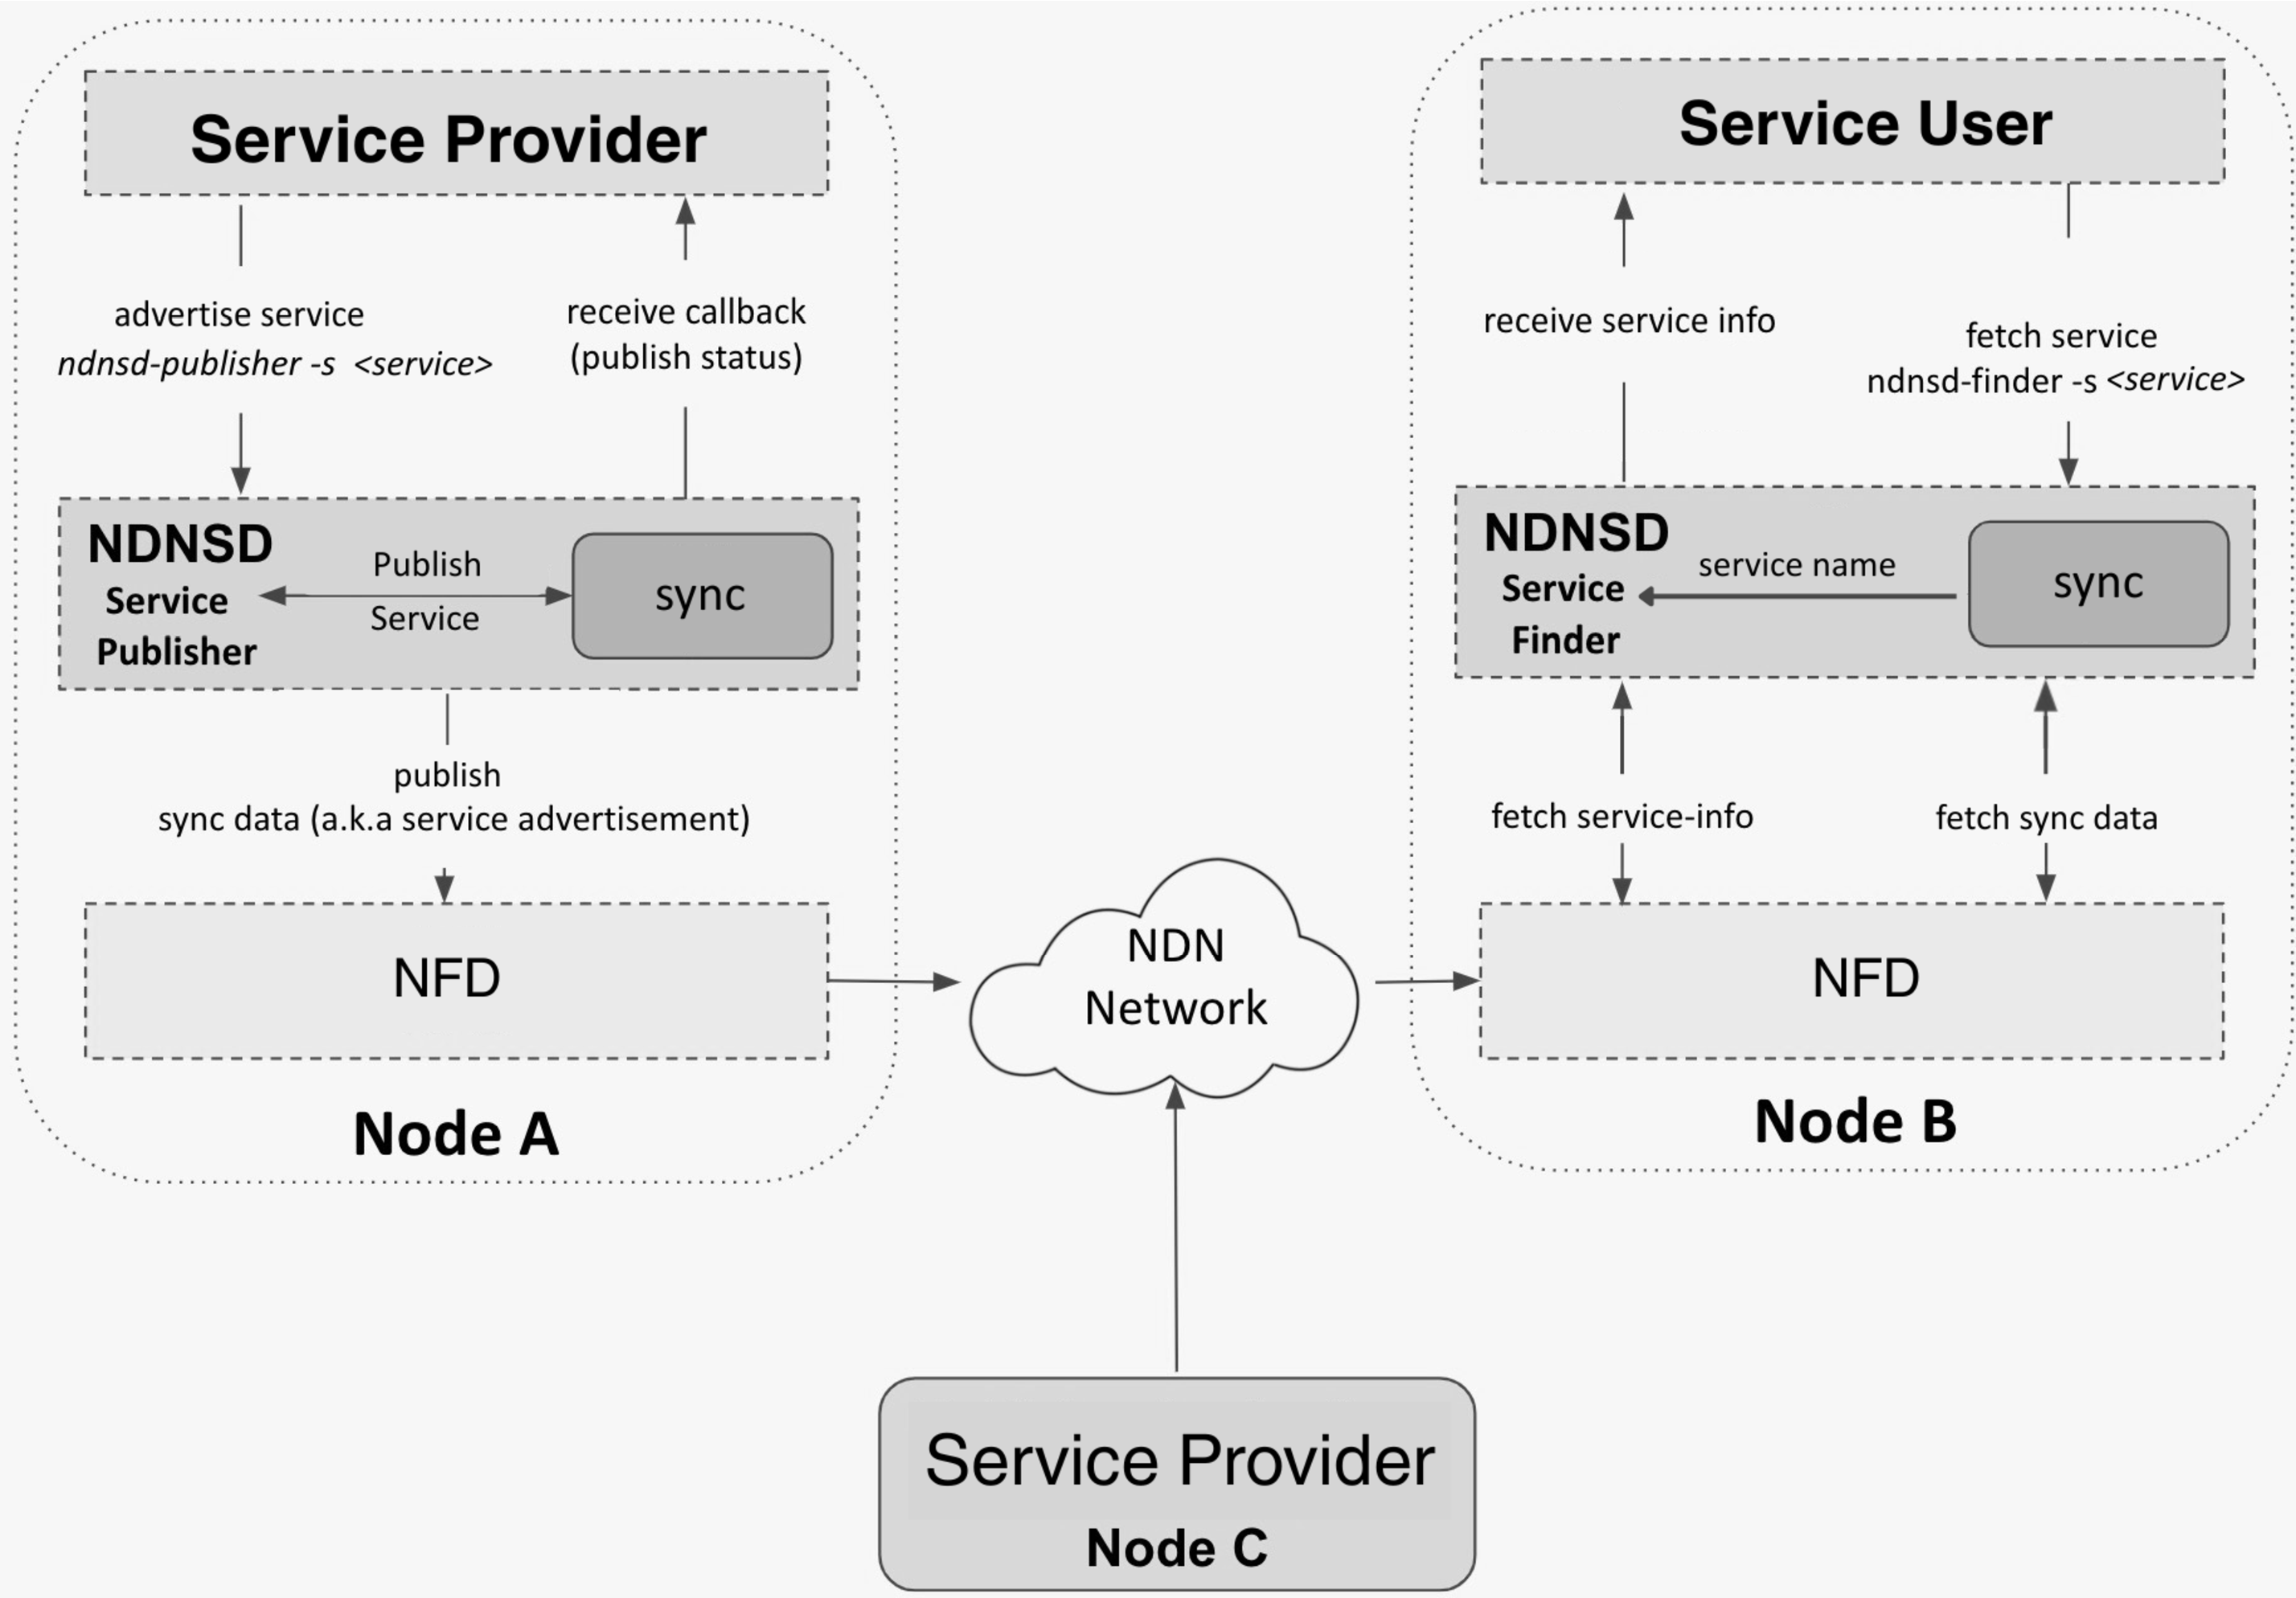
\includegraphics[width=\columnwidth]{figures/ndnsd.pdf}
    \caption{Service Publication and Discovery with NDNSD (adapted from~\cite{dulal2022ndnsd}, Fig.~2)}
    \vspace{-3mm}
    \label{fig:NDNSD}
\end{figure}

NDNSF can also use NDNSD~\cite{dulal2022ndnsd} to publish and discover service information before invocation. As shown in Figure~\ref{fig:NDNSD}, service providers publish their service information via NDN Sync (Section~\ref{sec:background}), allowing other participants in the Sync group (e.g., service users) to discover available services. NDNSD requires a service name and service-information lifetime; applications can add fields such as the provider's name prefix and a description. For example, a drone may publish the following information for its service:
\begin{quote}
Service Name: \texttt{/UAVNET/ImageProc/YOLO12}

Provider Name Prefix: \texttt{/UAVNET/drone2}

ServiceInfo Lifetime: \texttt{60s}

Description: \texttt{Real-time object detection service using YOLOv12}
\end{quote}
Advertisements help applications identify potential providers before issuing a request. Previously published information may remain retrievable from other available copies even when its provider is offline. However, an advertisement does not establish the provider's current availability or willingness to execute a particular task.

An application that has already chosen a provider can use targeted invocation (Section~\ref{sec:targeted-invocation}).

\subsection{Service Controller and Access Control}
\label{sec:service-controller}

\begin{figure*}[t]
\centering 

\begin{minipage}[c]{0.63\textwidth}
    \centering
    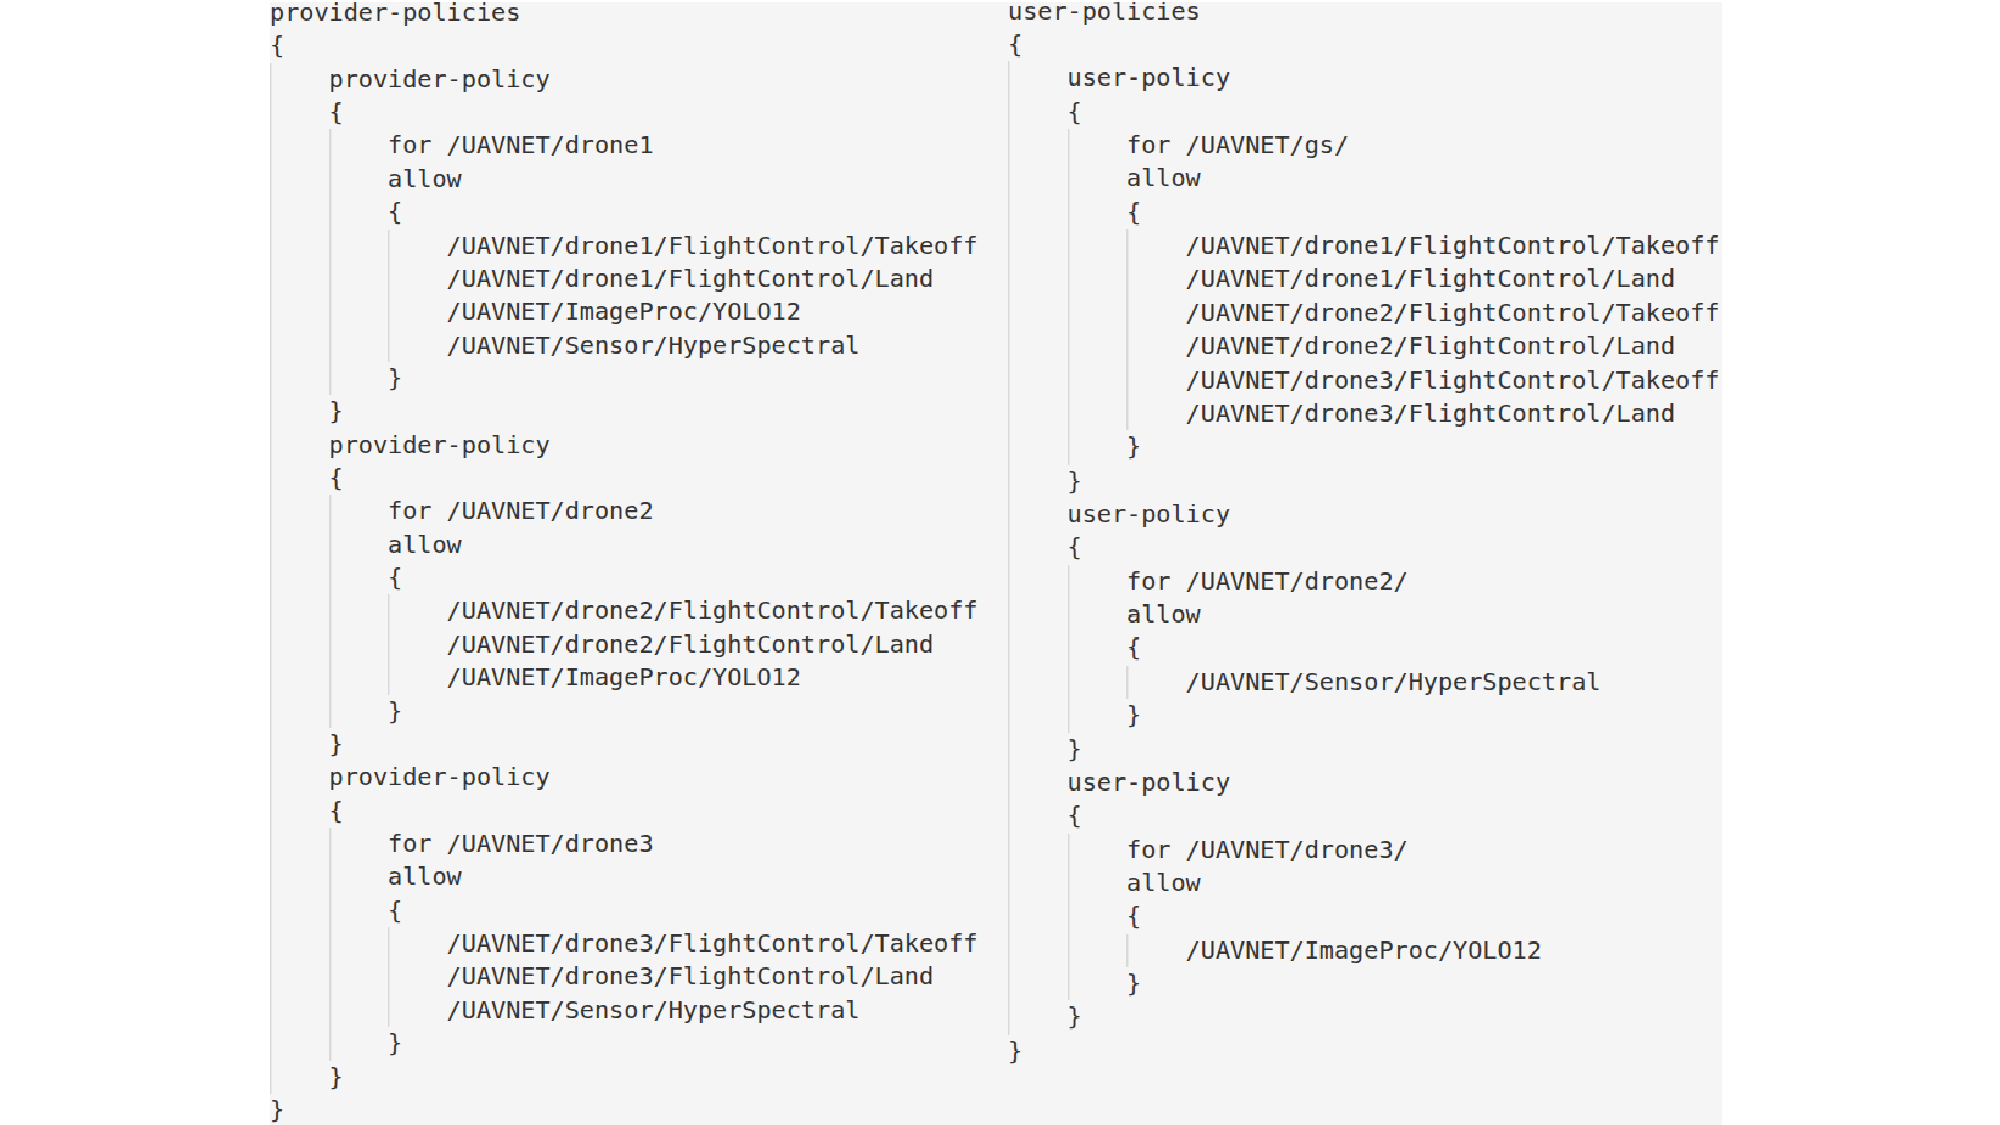
\includegraphics[width=\linewidth]{figures/user-provider-policy.pdf}
    \caption{An Example of Access Control Policies}
    \label{fig:PolicyExample}
\end{minipage}
\hfill
\begin{minipage}[c]{0.35\textwidth}
\centering

    % --- ROW 1: Request & ACK ---
    \begin{subfigure}[t]{0.49\linewidth}
    \centering
    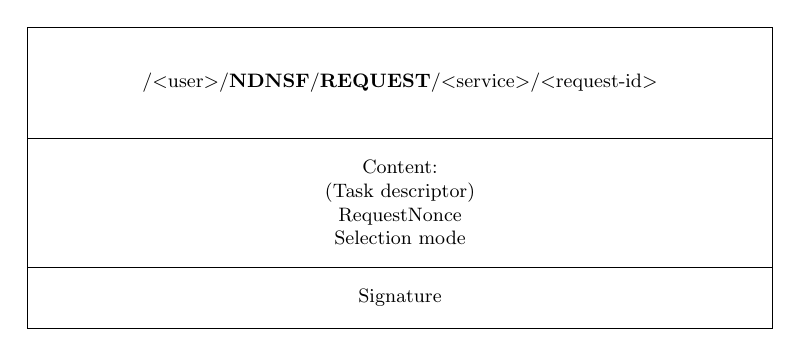
\begin{tikzpicture}[scale=0.78, transform shape]
    \def\W{1.0\linewidth} 
    \def\Hname{1.8}    % Vertically shrunk from 2.6
    \def\Hcontent{2.1} % Vertically shrunk from 2.2
    \def\Hsig{1.0}
    
    \useasboundingbox (0,0) rectangle (\W,\Hname+\Hcontent+\Hsig);
    \draw (0,0) rectangle (\W,\Hname+\Hcontent+\Hsig);
    \draw (0,\Hsig) -- (\W,\Hsig);
    \draw (0,\Hsig+\Hcontent) -- (\W,\Hsig+\Hcontent);
    
    \node[align=center, text width=0.95*\W, font=\small, inner sep=1pt] at (0.5*\W,\Hsig+\Hcontent+\Hname/2) {/$<$user$>$/\textbf{\allowbreak NDNSF}/\textbf{\allowbreak REQUEST}/\allowbreak $<$service$>$/\allowbreak $<$request-id$>$};
    \node[align=center, text width=0.95*\W, font=\small, inner sep=1pt] at (0.5*\W,\Hsig+\Hcontent/2) {Content:\\(Task descriptor)\\RequestNonce\\Selection mode};
    \node[font=\small] at (0.5*\W,\Hsig/2) {Signature};
    \end{tikzpicture}
    \caption{Request}
    \end{subfigure}%
    \hfill
    \begin{subfigure}[t]{0.49\linewidth}
    \centering
    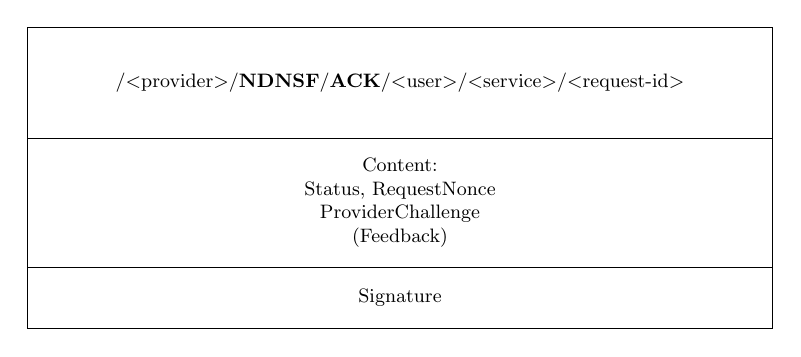
\begin{tikzpicture}[scale=0.78, transform shape]
    \def\W{1.0\linewidth}
    \def\Hname{1.8}    % Vertically shrunk from 2.6
    \def\Hcontent{2.1} % Vertically shrunk from 2.2
    \def\Hsig{1.0}
    
    \useasboundingbox (0,0) rectangle (\W,\Hname+\Hcontent+\Hsig);
    \draw (0,0) rectangle (\W,\Hname+\Hcontent+\Hsig);
    \draw (0,\Hsig) -- (\W,\Hsig);
    \draw (0,\Hsig+\Hcontent) -- (\W,\Hsig+\Hcontent);
    
    \node[align=center, text width=0.95*\W, font=\small, inner sep=1pt] at (0.5*\W,\Hsig+\Hcontent+\Hname/2) {/$<$provider$>$/\textbf{\allowbreak NDNSF}/\textbf{\allowbreak ACK}/\allowbreak $<$user$>$/\allowbreak $<$service$>$/\allowbreak $<$request-id$>$};
    \node[align=center, text width=0.95*\W, font=\small, inner sep=1pt] at (0.5*\W,\Hsig+\Hcontent/2) {Content:\\Status, RequestNonce\\ProviderChallenge\\(Feedback)};
    \node[font=\small] at (0.5*\W,\Hsig/2) {Signature};
    \end{tikzpicture}
    \caption{ACK}
    \end{subfigure}
    
    \vspace{6mm} 
    
    % --- ROW 2: Selection & Response ---
    \begin{subfigure}[t]{0.49\linewidth}
    \centering
    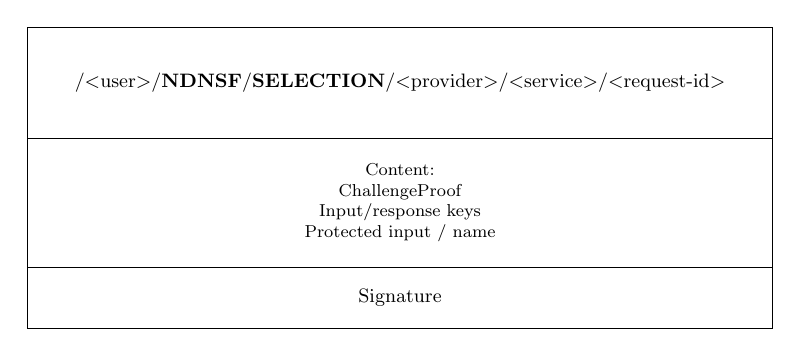
\begin{tikzpicture}[scale=0.78, transform shape]
    \def\W{1.0\linewidth}
    \def\Hname{1.8}    % Vertically shrunk from 2.6
    \def\Hcontent{2.1} % Vertically shrunk from 2.2
    \def\Hsig{1.0}
    
    \useasboundingbox (0,0) rectangle (\W,\Hname+\Hcontent+\Hsig);
    \draw (0,0) rectangle (\W,\Hname+\Hcontent+\Hsig);
    \draw (0,\Hsig) -- (\W,\Hsig);
    \draw (0,\Hsig+\Hcontent) -- (\W,\Hsig+\Hcontent);
    
    \node[align=center, text width=0.95*\W, font=\small, inner sep=1pt] at (0.5*\W,\Hsig+\Hcontent+\Hname/2) {/$<$user$>$/\textbf{\allowbreak NDNSF}/\textbf{\allowbreak SELECTION}/\allowbreak $<$provider$>$/\allowbreak $<$service$>$/\allowbreak $<$request-id$>$};
    \node[align=center, text width=0.95*\W, font=\footnotesize, inner sep=1pt] at (0.5*\W,\Hsig+\Hcontent/2) {Content:\\ChallengeProof\\Input/response keys\\Protected input / name};
    \node[font=\small] at (0.5*\W,\Hsig/2) {Signature};
    \end{tikzpicture}
    \caption{Selection}
    \end{subfigure}%
    \hfill
    \begin{subfigure}[t]{0.49\linewidth}
    \centering
    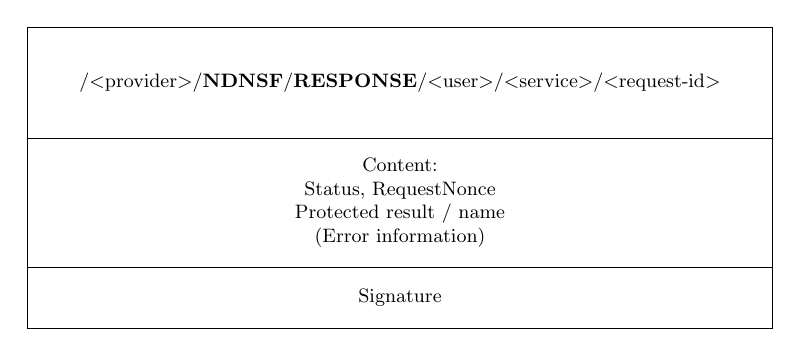
\begin{tikzpicture}[scale=0.78, transform shape]
    \def\W{1.0\linewidth}
    \def\Hname{1.8}    % Vertically shrunk from 2.6
    \def\Hcontent{2.1} % Vertically shrunk from 2.2
    \def\Hsig{1.0}
    
    \useasboundingbox (0,0) rectangle (\W,\Hname+\Hcontent+\Hsig);
    \draw (0,0) rectangle (\W,\Hname+\Hcontent+\Hsig);
    \draw (0,\Hsig) -- (\W,\Hsig);
    \draw (0,\Hsig+\Hcontent) -- (\W,\Hsig+\Hcontent);
    
    \node[align=center, text width=0.95*\W, font=\small, inner sep=1pt] at (0.5*\W,\Hsig+\Hcontent+\Hname/2) {/$<$provider$>$/\textbf{\allowbreak NDNSF}/\textbf{\allowbreak RESPONSE}/\allowbreak $<$user$>$/\allowbreak $<$service$>$/\allowbreak $<$request-id$>$};
    \node[align=center, text width=0.95*\W, font=\small, inner sep=1pt] at (0.5*\W,\Hsig+\Hcontent/2) {Content:\\Status, RequestNonce\\Protected result / name\\(Error information)};
    \node[font=\small] at (0.5*\W,\Hsig/2) {Signature};
    \end{tikzpicture}
    \caption{Response}
    \end{subfigure}

\caption{Principal fields of NDNSF's four invocation message types. ACK illustrates a positive reply; parentheses mark optional fields. Names are schematic; protection metadata and extensions are omitted.}
\label{fig:ndnsf-message-formats}
\end{minipage}
\end{figure*}


The \textbf{Service Controller} manages access control policies for providers and users. Provider policies specify which services an entity may offer, while user policies define which services it may access. These policies are designed to be simple and intuitive by leveraging NDN naming semantics. As shown on the left side of Figure~\ref{fig:PolicyExample}, drones 1-3 are authorized to provide their own flight-control services ending in \texttt{/FlightControl/Takeoff} and \texttt{/FlightControl/Land}. In addition, Drone~1 and Drone~2 may offer the image-processing service \texttt{/UAVNET/ImageProc/YOLO12}, while Drone~1 and Drone~3 may provide the sensing service \texttt{/UAVNET/Sensor/HyperSpectral}. The right side of the figure shows the corresponding user policies: the ground station \texttt{/UAVNET/gs} may access the flight-control services of all three drones, Drone~2 may access the hyperspectral sensing service, and Drone~3 may access the image-processing service.

Access control policies are translated into logical combinations of ABE attributes. NDNSF uses \textbf{service attributes} (\texttt{/SERVICE/<service-name>}) and \textbf{permission attributes} (\texttt{/PERMISSION/<service-name>}) to represent provisioning and access rights, respectively.  Here, \texttt{<service-name>} is a hierarchical NDN name consisting of one or more components that identify either a common service offered by multiple providers, a provider-specific service, or even a function within a service. These attributes encrypt service messages to control access (Section~\ref{sec:messages}). Under one ABE authority and the same set of public parameters, one DKEY can encode multiple service permissions. The naming hierarchy alone does not grant access to all services under a prefix; the ABE policy must encode the intended permissions.

\begin{figure}
    \centering
    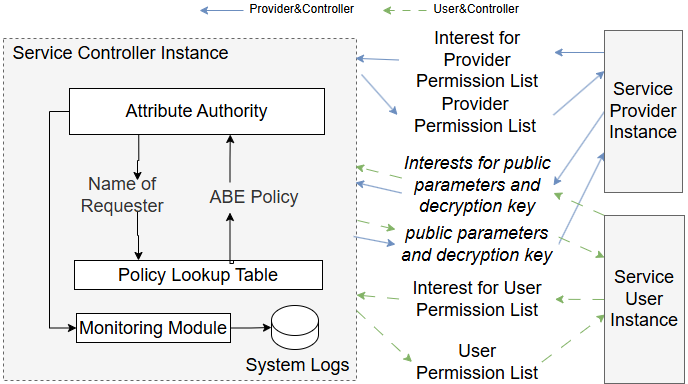
\includegraphics[width=.9\columnwidth]{figures/NDNSF_ServiceController.png}
    \caption{NDNSF Service Controller}
    \label{fig:ServiceController}
\end{figure}


%\begin{figure}[]
%\centering
%\begin{subfigure}[t]{0.25\textwidth}
%    \centering
%    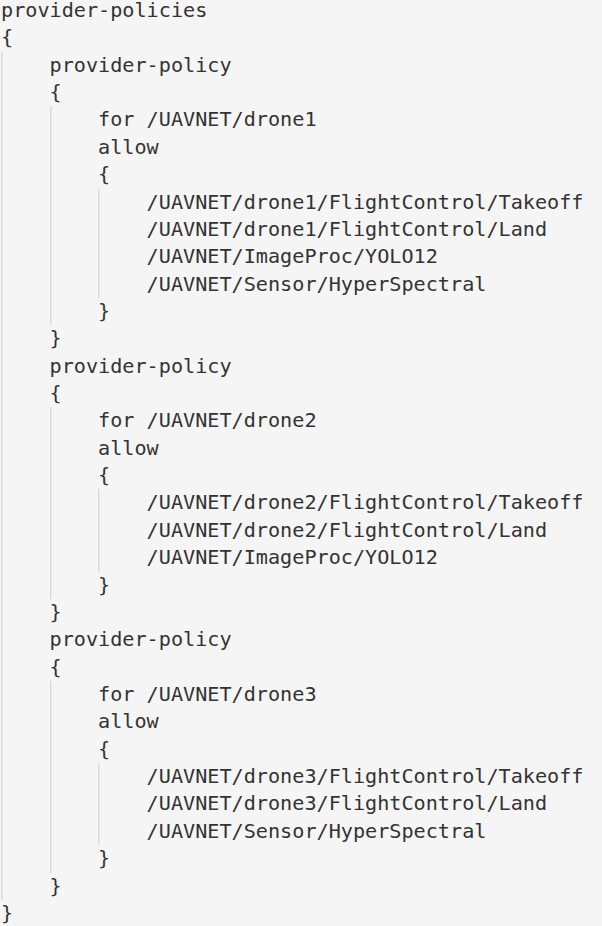
\includegraphics[width=\linewidth]{figures/Provider-policies.png}
%    \caption{Provider policies}
%\end{subfigure}
%\hfill
%\begin{subfigure}[t]{0.25\textwidth}
%    \centering
%    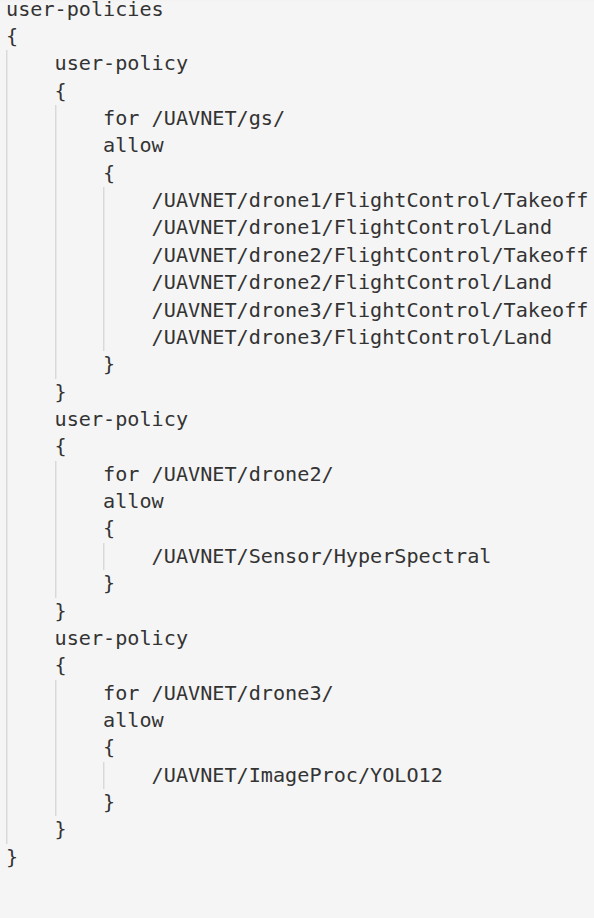
\includegraphics[width=\linewidth]{figures/User-policies.png}
%    \caption{User policies}
%\end{subfigure}
%\caption{An Example of Access Control Policies}
%\vspace{-3mm}
%\label{fig:PolicyExample}
%\end{figure}


The deployment administrator determines service permissions, and the Service Controller participates during onboarding and policy updates. As shown in Figure~\ref{fig:ServiceController}, inside the controller, the \textbf{Attribute Authority} maps an entity's name to its policy in the \textbf{Policy Lookup Table} and generates a decryption key (DKEY) that enables access to data encrypted under the corresponding attributes. The controller then securely distributes each entity's DKEY encrypted with the entity's public key. Through Interest--Data exchanges, users retrieve from the controller a \emph{User Permission List} specifying accessible services, while providers retrieve a \emph{Provider Permission List} specifying the services they are authorized to offer.

%Overall, NDNSF enables fine-grained, name-based access control over both service providers and users. By combining ABE with hierarchical NDN names, NDNSF achieves greater flexibility and scalability than traditional RBAC systems, while requiring only a single DKEY per entity regardless of the number of permissions.

\begin{comment}
\subsection{Service Provider and User}

\begin{figure}
    \centering
    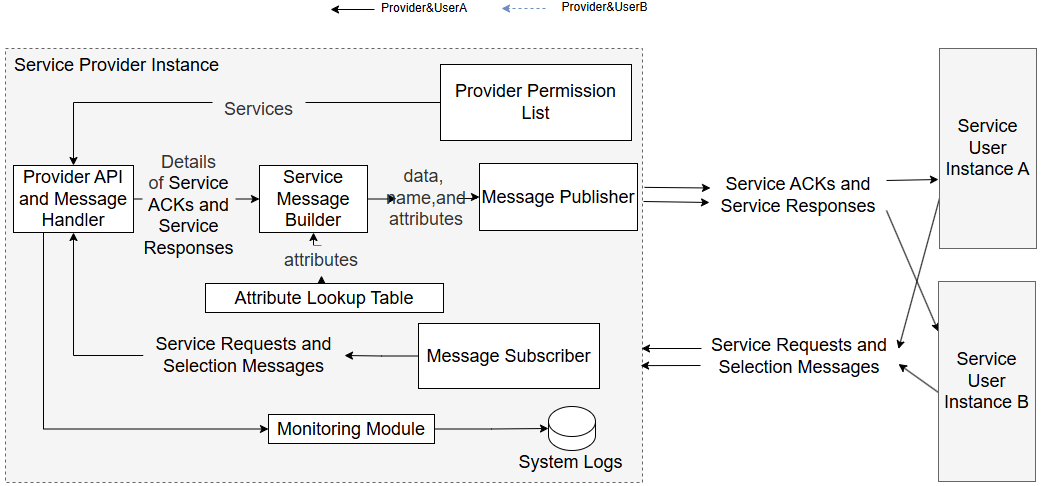
\includegraphics[width=\columnwidth]{figures/NDNSF_ServiceProvider.png}
    \caption{NDNSF Service Provider}
    \label{fig:ServiceProvider}
    \vspace{-3mm}
\end{figure}

As shown in Figure~\ref{fig:ServiceProvider}, each \textbf{Service Provider} runs a Subscriber Module to receive messages from Service Users and the Service Controller. The Service Message Builder generates response messages from processed requests and forwards them, together with the corresponding NDN names and attributes, to the Message Publisher, which creates encrypted NDN Data objects and advertises their names via Sync (Section~\ref{sec:messages}).

Figure~\ref{fig:ServiceUser} shows that each \textbf{Service User} runs a Subscriber Module to receive messages from Service Providers and the Service Controller; its remaining modules are analogous to those of the Service Provider.

\begin{figure}
    \centering
    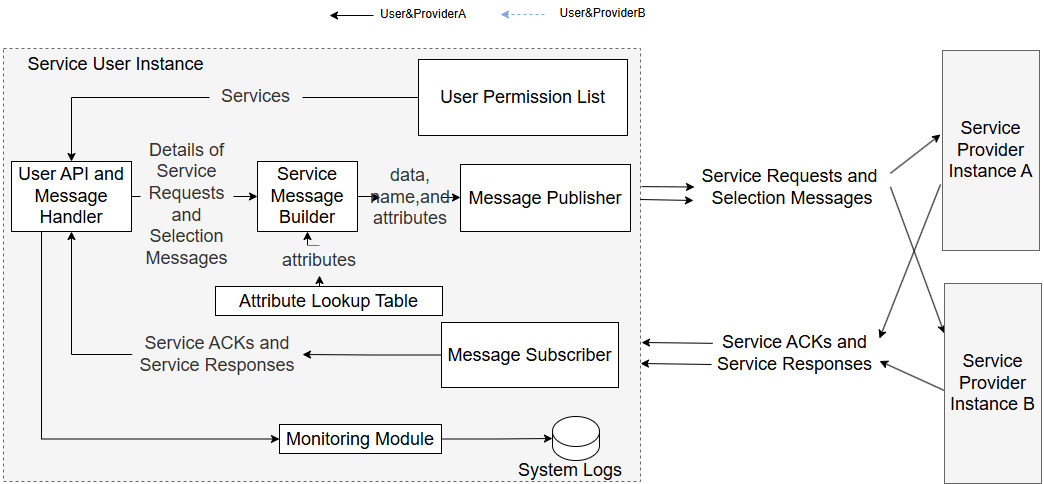
\includegraphics[width=\columnwidth]{figures/NDNSF_ServiceUser.png}
    \caption{NDNSF Service User}
    \vspace{-3mm}
    \label{fig:ServiceUser}
\end{figure}

\end{comment}

\subsection{Service Messages and Secure Communication}
\label{sec:messages}

As shown in Figure~\ref{fig:ndnsf-message-formats}, NDNSF defines four service message types---\emph{Request}, \emph{ACK}, \emph{Selection}, and \emph{Response}---each published as an NDN Data object containing a name, content, and signature. Service Users and Providers publish messages under their namespaces, announce publications through Sync, and subscribe to the messages they are responsible for processing. In the four-message flow, the Request message is one-to-many, while the remaining messages are one-to-one. The names in the figure are schematic: service names and request IDs may occupy multiple components, while an addressed participant's name occupies one encoded component.

A \textbf{Request Message} invokes a service from one or more providers. Its name follows \path{/<user>/NDNSF/REQUEST/<service>/<request-id>}, identifying the requester, the target service, and a request ID for response matching. The content includes an optional task descriptor specifying task requirements, a fresh \emph{RequestNonce}, and the provider-selection mode, all encrypted under the service attribute. Providers return the RequestNonce in subsequent ACK and Response messages to bind them to this request. The input and response keys are specific to each invocation (request-scoped protection). The task input is encrypted and delivered after selection, with its key shared only with selected providers in the Selection message.

Upon receiving a Request Message, each authorized provider decides whether to respond based on requested resources and performance requirements (Section~\ref{sec:provider-acknowledgment}). If accepted, it publishes an \textbf{ACK Message} named \path{/<provider>/NDNSF/ACK/<user>/<service>/<request-id>}. The ACK content carries the decrypted \emph{RequestNonce}, a fresh \emph{ProviderChallenge}, and optional \emph{AckMetaData}, encrypted under the permission attribute. \emph{AckMetaData} can include the number of requests in the provider's task queue or other information that may help the user select providers, e.g., resources the provider can dedicate to this request. The ACK may also identify the Provider's encryption key.

After receiving one or more ACK messages, the user issues one or more \textbf{Selection Messages} according to the provider-selection strategy (Section~\ref{sec:provider-selection}). The message name follows \path{/<user>/NDNSF/SELECTION/<provider>/<service>/<request-id>}. Its content is encrypted under the service attribute and includes a \emph{ChallengeProof} derived from the ProviderChallenge. It also carries the protected input or its Data name. The input and response keys are encrypted for the selected Provider and included in the Selection message. The Provider checks the proof and verifies that the Selection matches the request before execution.

Finally, each selected provider returns a \textbf{Response Message}, named \path{/<provider>/NDNSF/RESPONSE/<user>/<service>/<request-id>}, containing status, the protected service result or its Data name, and the \emph{RequestNonce}. The content is encrypted under the permission attribute. Decrypting the result also requires this invocation's response key; permission to read the outer message alone is insufficient. Larger input and result objects are published separately under their Producers' names.

% Addendum to the existing service-message discussion; preserve section numbering.
\label{sec:security-boundaries}
\textbf{Authorization scope and credential reuse.} ABE restricts descriptor access to entities whose DKEY policies permit decryption, including authorized providers that are not selected. Names and traffic patterns remain visible. ACK and Response content encrypted only for a service permission can also be read by other holders of that permission.

ABE policies carry service permissions, allowing baseline trust rules to focus on identity and message-signing relationships rather than per-entity service-permission lists. Identity credentials and these rules can be reused across applications sharing the same identity trust configuration. Trust rules still specify which keys may sign each message type~\cite{yu2015trust}; when processing Selection, providers must also check that it comes from the requesting user, refers to the same service and request, contains the stored provider challenge, and is allowed by the current request state. Rejecting replay requires tracking whether the request has expired or the challenge has already been used. Issuing a replacement DKEY does not invalidate an old DKEY retained by its holder. Revocation requires key rotation or additional permission checks and cannot prevent use of previously disclosed plaintext.


Table~\ref{tab:message-acceptance} summarizes the checks required by the basic invocation flow. All four message types require signature validation, an authorized signing key for the message name, and consistent service and request identifiers. The challenge checks assume that authorized participants do not disclose protected values to unauthorized parties. The invocation experiments do not independently test every rejection condition.

\begin{table*}[t]
\centering
\caption{Acceptance checks for basic invocation messages}
\label{tab:message-acceptance}
\small
\begin{tabularx}{\textwidth}{@{}lX@{}}
\toprule
Message & Additional checks before advancing the invocation \\
\midrule
Request & The provider can decrypt content protected for the requested service, and evaluates whether to participate. A duplicate request must not create a conflicting challenge or execution. \\
ACK & The user matches RequestNonce to its active request and associates the feedback and ProviderChallenge with the signing provider. Only positive ACKs passing these checks supply candidates for selection. \\
Selection & The provider matches the requesting user, service, request, and stored ProviderChallenge. The request must still permit execution, and a repeated Selection must not start a second execution. \\
Response & The user matches RequestNonce, the active request, and a selected provider. Duplicate or late results must not be accepted as results of another request. \\
\bottomrule
\end{tabularx}
\end{table*}


\subsection{Targeted Invocation}
\label{sec:targeted-invocation}

As a special case, an application that has preselected a Provider can name it in a targeted Request, for example to start a task on \texttt{drone1} or change that drone's flight-control setpoint. Targeted invocation does not substitute another device when the target is unavailable.

The Provider prepares pairs of requester and provider challenges for subsequent calls. When a valid, unused pair is available, the call can use only Request and Response; otherwise ACK and Selection must be exchanged first. The authorization, request-binding, and input-protection requirements of Section~\ref{sec:messages} still apply. Avoiding a new ACK--Selection exchange reduces repeated-call delay (Appendix~\ref{sec:targeted-invocation-evaluation}), but does not guarantee a flight-control deadline.


\subsection{Message Recovery and Timeout Handling}
\label{sec:loss-timeout}

NDNSF handles packet loss at two layers. At the synchronization and retrieval layer, NDN-SVS synchronizes publication state and retries retrieval of missing Data~\cite{moll2021svs,ndnsvs-github}. These retries aim to recover service messages without initiating a new service invocation.

At the invocation layer, NDNSF's data-driven workflow advances only when the required Data arrives and passes the applicable checks: in the four-message flow, ACK Data enables provider selection and Selection Data enables execution; Response Data delivers the result. An eligible targeted call instead uses the cached challenge material described in Section~\ref{sec:targeted-invocation} and does not wait for ACK or Selection. Request timers and, where applicable, ACK-collection timers continue to run during retrieval retries, so a recovered message may arrive too late to be used in that invocation.

If no result is accepted, the request timer triggers timeout handling. A grace interval after observed progress (500\,ms by default) and event-loop scheduling can extend acceptance beyond the configured timeout. The application decides whether to issue a new request, but a timeout does not prove that the provider did not execute the task. Retrying operations such as flight commands can therefore cause duplicate effects.

%This integrated naming, content, and encryption design ensures that NDNSF messages are not exposed to unauthorized entities while simultaneously achieving bidirectional authorization. The use of encrypted RequestNonces and one-time service tokens binds message semantics to cryptographic verification, preventing unauthorized participation and mitigating replay attacks. Even if an adversary replays previously captured messages, expired or invalid tokens will not be accepted, thereby preserving the correctness and stability of the system.

\subsection{ACK Strategy}
\label{sec:provider-acknowledgment}

In NDNSF, each provider makes a decision on whether to respond to a service request based on requested resources and performance requirements. The requested resources may include CPU/GPU, memory, trusted execution environments, and bandwidth. Performance requirements may further include response time and computation accuracy level. A provider publishes a positive ACK when its application-defined strategy accepts the task; this reports willingness to participate, without reserving resources or guaranteeing that the requirements will still be met when execution begins.
%This mechanism mitigates resource exhaustion, reduces unnecessary waiting time, and improves system stability. 

\subsection{Provider Selection Strategy}
\label{sec:provider-selection}

\begin{figure}
    \centering
    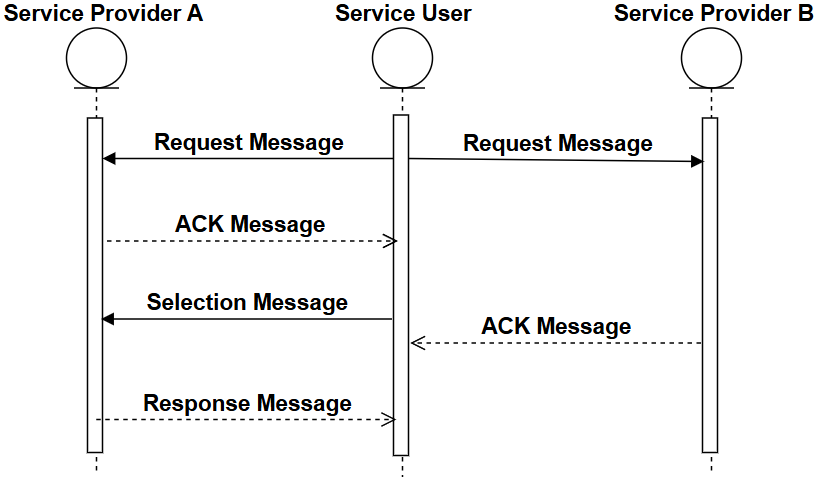
\includegraphics[width=.9\columnwidth]{figures/First-Responding.png}
    \caption{First-Responding Strategy}
    \label{fig:First-Responding}
\end{figure}

\begin{figure}
    \centering
    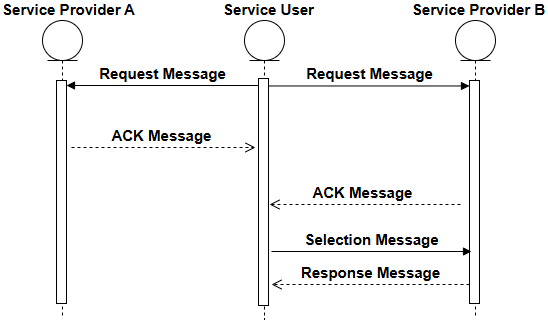
\includegraphics[width=.9\columnwidth]{figures/Random-Selection.png}
    \caption{Random-Selection Strategy}
    \label{fig:Random-Selection}
\end{figure}

\begin{figure}
    \centering
    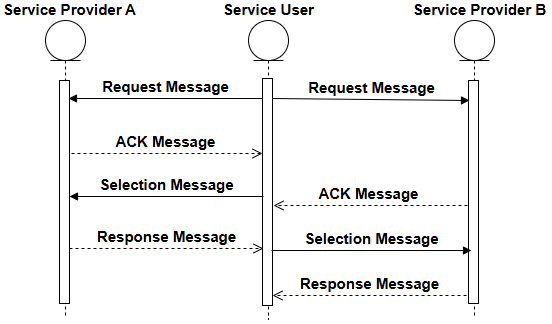
\includegraphics[width=.9\columnwidth]{figures/All-Responders.png}
    \caption{All-Responders Strategy}
    \label{fig:All-Responders}
\end{figure}

When multiple service providers offer the same service, NDNSF enables the user to select one or more providers for execution. It supports three built-in provider selection strategies, as well as user-defined custom strategies, allowing optimization based on metrics such as RTT, computational capacity, bandwidth, or other application-specific requirements. Candidates must return positive ACKs that pass the applicable message and authorization checks.
\begin{enumerate}
\item \textbf{First-Responding Strategy (Figure~\ref{fig:First-Responding})}: the user selects the first provider that returns a valid ACK. For example, if Drone~1 and Drone~2 both offer the \texttt{YOLO12} service and Drone~1 responds first, Drone~1 is selected.
\item \textbf{Random-Selection Strategy (Figure~\ref{fig:Random-Selection})}: when the ACK-collection window closes, the user randomly selects one provider from the collected valid ACKs. This is suitable for load balancing among similar providers.
\item \textbf{All-Responders Strategy (Figure~\ref{fig:All-Responders})}: all providers whose valid ACKs are collected before the window closes are selected to execute the service. This is intended for redundancy or cross-validation, e.g., multiple drones independently sensing the same target.
\item \textbf{Custom-Selection Strategy}: NDNSF also supports user-defined provider-selection strategies based on published service information, application-supplied runtime measurements, and optional metadata included in ACK messages by providers (e.g., resource availability and processing cost).
\end{enumerate}
For strategies that collect ACKs, the window may close early when the reply count reaches the recently observed provider count, reducing wait while excluding later ACKs.
\subsection{NDNSF Application Programming Interface}
\label{sec:NDNSF-API}

\begin{figure}[]
\centering

% --- Top Listing: Provider-Side API ---
\begin{lstlisting}[
    style=ndnsfstyle,
    language=C++,
    caption={Provider-Side API},
    label={lst:provider-api}
]
void Provider::addService(
    ServiceName service,
    AckHandler onAck,
    RequestHandler onRequest
);
\end{lstlisting}

\vspace{4mm} % Adds a clean breathing gap between the two blocks

% --- Bottom Listing: User-Side API ---
\begin{lstlisting}[
    style=ndnsfstyle,
    language=C++,
    caption={User-Side API},
    label={lst:async-call}
]
RequestId User::RequestService(
    ServiceName service,
    RequestPayload request,
    int ackCollectionTimeMs,
    AckSelectionPolicy selectionPolicy,
    int timeoutMs,
    ResponseCallback onResponse,
    TimeoutCallback onTimeout
);
\end{lstlisting}

\caption{Simplified APIs for the four-message invocation flow}
\label{fig:ndnsf-apis}
\end{figure}

Figure~\ref{fig:ndnsf-apis} summarizes the invocation API using simplified types.

%LW: does the provider call this only one time for all the incoming requests
\texttt{addService} registers a named service together with two callbacks, \texttt{onAck} and \texttt{onRequest}. In the four-message flow, the \texttt{onAck} callback is invoked when a request is received, allowing the provider to decide whether to serve the request and optionally include metadata in its ACK. The \texttt{onRequest} callback is invoked after the user selects the provider and sends a Selection message; an eligible targeted call can reach execution without a new Selection exchange. This two-stage flow enables informed decision making by both providers and users.

%LW: what if there are multiple responses?
\texttt{RequestService} is the primary user-side service invocation interface. The application specifies the service name and request payload, without explicitly identifying providers. It also supplies two timeout values, a \texttt{selectionPolicy}, and two callbacks, \texttt{onResponse} and \texttt{onTimeout}. NDNSF publishes the request to solicit eligible providers and uses \texttt{ackCollectionTimeMs} to configure the ACK-collection window. It applies the policy as ACKs arrive or when the window closes. Accepted responses are delivered to \texttt{onResponse}; request expiration is handled by \texttt{onTimeout} as described in Section~\ref{sec:loss-timeout}.

For a service registered to support targeted invocation, \texttt{RequestServiceTargeted} takes the provider name, service name, request, timeout and timeout/response callbacks. The application supplies the target; the framework applies the authorization checks and challenge-pair rules described in Section~\ref{sec:targeted-invocation}.


\section{IMPLEMENTATION}
%TODO: cite the correct code
\label{sec:impl}
NDNSF was implemented using \texttt{ndn-cxx}~\cite{ndn-cxx}, NDN-SVS~\cite{ndnsvs-github}, and NAC-ABE~\cite{dulal2023nac-abe}.

NDNSF validates certificate chains against fixed trust anchors, checks certificate validity periods, and enforces configured application trust rules. Cached certificate validation expires with the validated chain.

For NAC-ABE, cached keys avoid repeated retrieval and decryption. Small publications can also be carried directly in Sync Interest Application Parameters, avoiding a separate publication fetch. Regular-expression subscriptions filter message types and Request service names; receivers then check the recipient, service and invocation bindings.

Peers can reference immutable, producer-signed security profiles by exact Data name under the Producers' prefixes. Receivers fetch and validate uncached profiles, reuse their encryption certificates and capabilities within certificate validity, and retain authorization and request-binding checks for each invocation.

SVS byte-publication preparation is synchronous by default; optional bounded workers can prepare publications asynchronously. Network operations remain on the Face event loop. The evaluation measures the combined invocation path rather than each optimization separately.

Request-scoped protection is enabled by default for Controller-managed calls. With custom capability settings, input and result isolation depends on retaining request-scoped protection.

A two-provider MiniNDN functional experiment verified protected nonempty input delivery and results for both selected providers; in a separate call, a nonselected provider did not obtain decrypted input or usable Selection keys. The performance experiments below select one provider per invocation.

%NDNSF was implemented using ndn-cxx~\cite{ndn-cxx}, NDN-SVS~\cite{ndnsvs-github}, and NAC-ABE~\cite{dulal2023nac-abe}. During development, we observed that the baseline NAC-ABE and NDN-SVS implementations did not adequately meet performance expectations, and we therefore introduced several optimizations.

%For NAC-ABE, we implemented a key-caching mechanism to eliminate repeated key retrieval and decryption, reducing decryption latency by approximately one RTT per operation. For NDN-SVS, messages smaller than 512~bytes are embedded in the Sync Interest’s Application Parameters, reducing the publication-to-reception delay by one RTT. In addition, to ensure that users and providers receive only relevant messages, we introduced a regular-expression-based subscription mode into NDN-SVS.
%For example, the user \path{/UAVNET/Drone3} requesting the \path{ImageProc/YOLO12} service uses the following two regular expressions in its subscriptions: \path{"<>+/<NDNSF>/<ACK>/<UAVNET>/<Drone3>/<ImageProc>/<YOLO12>/<>"} for ACK messages and \path{"<>+/<NDNSF>/<RESPONSE>/<UAVNET>/<Drone3>/<ImageProc>/<YOLO12>/<>"} for Response messages. On the other hand, the provider \path{/UAVNET/Drone1}, which offers the service \path{/UAVNET/ImageProc/Yolov12}, subscribes to Request messages using \path{"<>+<NDNSF><REQUEST><UAVNET><ImageProc><Yolov12><>"} and to Selection messages using \path{"<>+<NDNSF><SELECTION><UAVNET><Drone1><ImageProc><Yolov12><>"}.

%Finally, under high-frequency NDNSF workloads, the original blocking APIs and heavily single-threaded design of NDN-SVS became a major bottleneck, since most synchronization and processing logic executed on the main Face event loop. To address this issue, we redesigned Sync Interest handling and publication into an asynchronous pipeline. CPU-intensive tasks such as state-vector processing, decoding, comparison, and metadata preparation are offloaded to a bounded worker pool, while all NDN Face and \texttt{io\_context} operations remain on the main NDN thread to preserve thread safety. In addition, we introduced a nonblocking asynchronous publish path that prevents application-level request handling from stalling the Face event loop. These optimizations significantly improve NDNSF scalability and responsiveness under high-frequency request workloads.

%To demonstrate how NDNSF can be used to build distributed applications and evaluate its performance, we developed a UAV system demo in which the ground station invokes the Flight Control service provided by the drone. This demo utilizes NDNSF for inter-node communication and access control, and once the drone's onboard computer verifies the command, it uses the MAVSDK API to control the UAV flight controller, thereby enabling autonomous operation of the UAV.


\section{EVALUATION}
\label{sec:eval}

We first analyze credential-management costs, then evaluate service invocation against NSC~\cite{meirovitch2021nsc}, an NDN remote code execution framework, and gRPC, an IP-based remote procedure call framework. The invocation experiments examine reliability under loss and provider unavailability, followed by the effects of ACK and provider-selection strategies.

\subsection{Credential Management Costs}
\label{sec:credential-cost}

For the same permission assignments, let $N$ be the number of entities, each holding at least one service permission, $p$ the average number of service permissions per entity, and $r$ the average number of roles per entity for which separate credentials are issued. A role may cover multiple services. We count credentials held by entities, not distinct shared service-key values across the deployment.

\begin{table}[t]
\centering
\caption{Entity-held credentials under shared identity trust}
\label{tab:credential-counts}
\small
\begin{tabularx}{\columnwidth}{@{}Xcc@{}}
\toprule
Credential category & NDNSF & Separate service keys \\
\midrule
Identity-signing credentials & $N$ & $N$ \\
Service-decryption credentials & $N$ & $Np$ \\
Subtotal & $2N$ & $N+Np$ \\
\bottomrule
\end{tabularx}
\end{table}

Table~\ref{tab:credential-counts} counts identity-signing and service-decryption credentials separately before adding them. Both configurations assume one active identity-signing credential per entity; a certificate and its associated private key are treated as one managed signing credential, not as one cryptographic key. NDNSF additionally assumes one ABE authority, one set of public parameters, and one current DKEY per entity. For 100 entities with 20 permissions each, the subtotals are 200 credentials for NDNSF and 2,100 for the separate-service-key configuration. These subtotals exclude content keys, additional encryption credentials, and authority-side material; any differences in those items must also be counted in a complete comparison.

Fewer credential objects do not necessarily mean fewer bytes or network messages. Let $L_i$ be the number of attribute occurrences in entity $i$'s access policy. For a construction whose key size grows linearly with $L_i$, total DKEY size is $\Theta(\sum_i L_i)$. If each policy lists its service permissions individually, this remains $\Theta(Np)$. DKEYs exceeding a Data packet's payload capacity require segmentation~\cite{dulal2023nac-abe}; separate-key deliveries can also be batched.

Granting another permission may require issuing a replacement DKEY containing the entity's updated policy. A separate-key design may instead deliver only the additional service key. Revocation that rotates the authority's parameters requires replacement DKEYs for every entity retaining permissions under that authority. Rotating only an affected service's shared key may require updates for fewer entities.

With a separately issued credential per assigned role, the role-credential count is $Nr$, or $\Theta(Nr)$. A role certificate may also be used to sign messages, so adding another $N$ identity credentials would double-count objects unless separate identity credentials are actually maintained. DNMP and trust schemas do not require a certificate per service~\cite{nichols2019dnmp,yu2015trust}; one role may cover several services. Role-based alternatives also need encryption for descriptor confidentiality, and those decryption credentials must be included when comparing complete configurations.

Aggregation reduces the number of decryption credentials to manage. Its overall cost depends on policy size, role reuse, and permission-change frequency.

\subsection{Trust-Rule Management Costs}
\label{sec:trust-rule-cost}

Trust-rule management must be counted separately from credential objects. DNMP compiles its VerSec schema into a signed binary representation for runtime use; its three-role prototype expresses the schema in 25 lines, excluding comments~\cite{nichols2019dnmp}. Parameterized rules can cover many identities, so neither DNMP nor NDNSF necessarily needs a separate trust rule for each entity or service permission.

Let $E$ denote the number of explicitly stored role--service authorization relationships. Listing these relationships requires $\Theta(E)$ entries, but does not imply $E$ independent schema rules: patterns or shared roles may express the same assignments more compactly. In NDNSF, individually listing each entity's service permissions requires $Np$ permission entries at the Controller, or $\Theta(Np)$, even though there are only $N$ DKEY objects. With fixed message formats and naming conventions, baseline signing rules in either design need not grow with $N$. NDNSF keeps service-permission lists in ABE policies; role-based designs can also change membership through credentials or authorization state without changing the schema. Changing a role's allowed actions may instead require a schema update.

For an update that delivers a complete $B$-byte signed schema to $V$ validators, the cumulative bytes received are $\Theta(VB)$. This is not the total network-link traffic, which depends on multicast, caching, and topology. A complete cost comparison must also include schema compilation, credential or DKEY updates, and permission-state distribution. Compilation and runtime validation costs must be measured separately; they cannot be inferred from credential or rule counts.

Keeping service-permission lists outside baseline signing rules does not eliminate permission-management costs; NDNSF manages them through ABE policies and keys. The invocation experiments do not measure key-distribution, schema-management, or revocation costs.


\subsection{Permission Aggregation: Measured Costs and Limits}
\label{sec:measured-permission-cost}

We compare eight identities with 1, 4 or 16 permissions under three C++ measurement configurations: one aggregated NAC-ABE DKEY per identity, separate NAC-ABE DKEYs per permission, and one RSA-protected bundle of AES service keys per identity. Five matched repetitions check authorized access, rejection of tampered data, rejection of new ciphertext by revoked holders retaining old keys, and surviving users' access after revocation.

At 16 permissions, initial local management CPU time, including key generation and recipient processing, is 303.10\,ms for aggregated ABE, 704.58\,ms for separate ABE keys and 6.15\,ms for batched RSA/AES. Aggregation lowers this cost relative to separate ABE keys, but the batched alternative has the lowest local cost in every measured phase.

A separate network comparison distributes pre-generated signed objects and excludes online generation. At 16 permissions, aggregation reduces initial management traffic from 281.72 to 86.74\,KiB relative to separate ABE keys (paired reduction 194.98\,KiB; 95\% interval 193.87--196.10), and revocation traffic from 247.11 to 75.80\,KiB. Eight aggregated DKEYs replace 128 separate DKEYs. At one permission, both ABE configurations use about 21.96\,KiB initially; a single new permission costs more under aggregation because it replaces a larger policy. The batched RSA/AES alternative uses only 27.25\,KiB initially and less traffic in every measured phase. Thus, aggregation helps relative to per-permission ABE when permissions are numerous, but is neither generally cheaper than batching nor free to update.

A separate MiniNDN~\cite{MININDN} experiment measures access recovery through the NDNSF Controller, Provider and User APIs, with five runs each at one and sixteen permissions per identity. All runs restore authorized access. At sixteen permissions, observed recovery takes 0.664--2.713\,s after a grant and 3.348--7.022\,s for the seven surviving users after revocation and key rotation. Calls using the pre-revocation permission state also complete after the revocation update, and some calls have no terminal result by the end of the observation window. These observations do not establish immediate revocation or uninterrupted service. This experiment does not compare management costs through the framework APIs across the three alternatives. Appendix~\ref{app:measured-permission-cost} gives the cost breakdown, reuse comparison and recovery details.

\subsection{Invocation Comparison Scope}

In the multi-provider comparisons with fixed-provider baselines, NSC and gRPC call one fixed provider, while NDNSF solicits several candidates and selects from their ACKs. NSC and NDNSF use signed NDN packets; NDNSF additionally uses NAC-ABE to protect service content. The matched multi-provider experiment below also enables failover in NSC and gRPC, but compares complete invocation paths rather than isolating feedback. These cross-framework comparisons do not isolate security overhead.
\subsection{Experimental Setup}

The original single-provider loss, fixed-provider, ACK-strategy, provider-selection, mobility and real-machine measurements used pre-provisioned certificates and excluded online certificate-chain retrieval and validation. They describe that implementation and do not quantify the current validation path. The no-loss single-provider and matched invocation studies use fixed-root certificate validation.

\begin{figure}[]
    \centering
    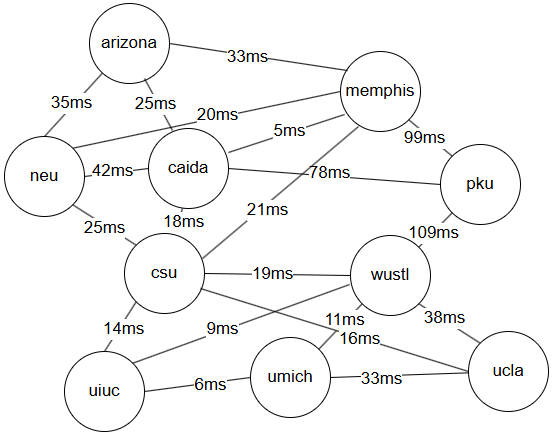
\includegraphics[width=0.4\textwidth]{figures/testbed_topo.png}
    \caption{Wired Network Topology}
    \label{fig:wired_topo}
    \vspace{-3mm}
\end{figure}

Figure~\ref{fig:wired_topo} illustrates the emulated wired network used in the wired invocation experiments unless otherwise specified, derived from a subset of the global NDN Testbed topology~\cite{testbedtopo}. All nodes are connected by 1~Gbps wired links, with per-link latency configured according to the values shown in the topology. Unless otherwise specified, all links are lossless; in lossy wired network experiments, a uniform packet loss rate of 1\% is applied to every link.

\begin{figure}[]
    \centering
    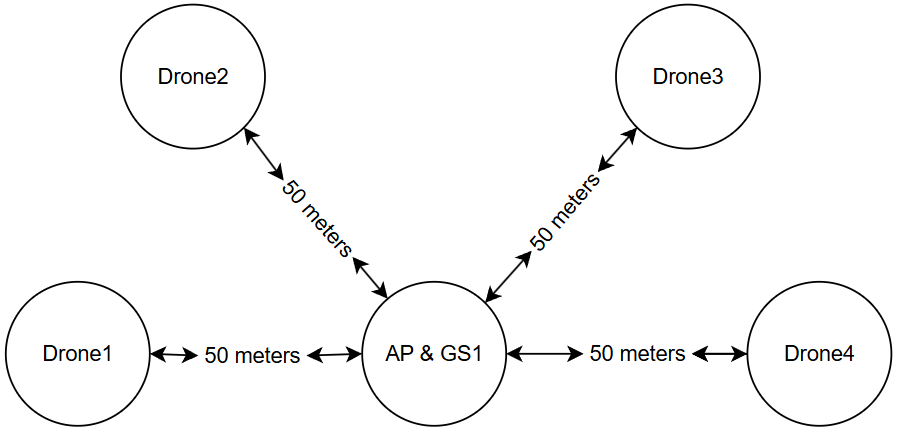
\includegraphics[width=0.4\textwidth]{figures/WIFI_TOPO.png}
    \caption{Wireless Network Topology}
    \label{fig:wifi_topo}
    \vspace{-3mm}
\end{figure}

Figure~\ref{fig:wifi_topo} depicts the emulated wireless network. All drones initially start 50~meters from the ground station and then move randomly within a 400\,m $\times$ 400\,m area centered at the ground station following the Random Waypoint mobility model. The WiFi access point (AP) is colocated with the ground station, and its communication range is varied across experiments. Drones moving outside the AP range cannot receive packets, resulting in mobility-induced packet loss.

In addition to the emulation experiments, we conduct real-world experiments using a Lenovo Y70 laptop, a desktop PC equipped with an AMD Ryzen 7 3700X processor, and an Odroid C4 device. The PC is connected directly to a WiFi AP over Ethernet, whereas the laptop and Odroid C4 communicate wirelessly through the same AP.

In the single-provider, fixed-provider, ACK-strategy, provider-selection, mobility and real-machine comparisons, NDNSF users employ the first-responding provider-selection strategy unless otherwise specified. By default, providers acknowledge and serve all incoming requests. Each service request incurs a 5\,ms processing delay at the provider to emulate service execution overhead. Except for the no-loss single-provider comparison, these experiments use a 512~B publication-embedding threshold, which limits the encoded Data size eligible for carriage in Sync Interests. The targeted, matched-availability, advertisement and permission studies specify their own workloads and completion criteria.
\subsection{Performance Metrics}

We use the following metrics in our evaluation:

\begin{enumerate}
\item \textbf{Service Latency}: the time interval from initiating a service request to receiving the service result.

\item \textbf{Success Rate}: the proportion of measured service requests for which the user accepts a result under the invocation's configured timeout handling. A request counts once, regardless of message retrieval retries. A timeout does not establish whether the provider executed the request.
\end{enumerate}

The single-provider, fixed-provider, ACK-strategy, provider-selection, mobility and real-machine comparisons report point estimates without repetition-based uncertainty estimates. They do not establish statistical differences or isolate authorization costs. The matched studies report repetitions and uncertainty.

\subsection{Wired Evaluation Results with One Provider}

\begin{figure}[!h]
  \centering
  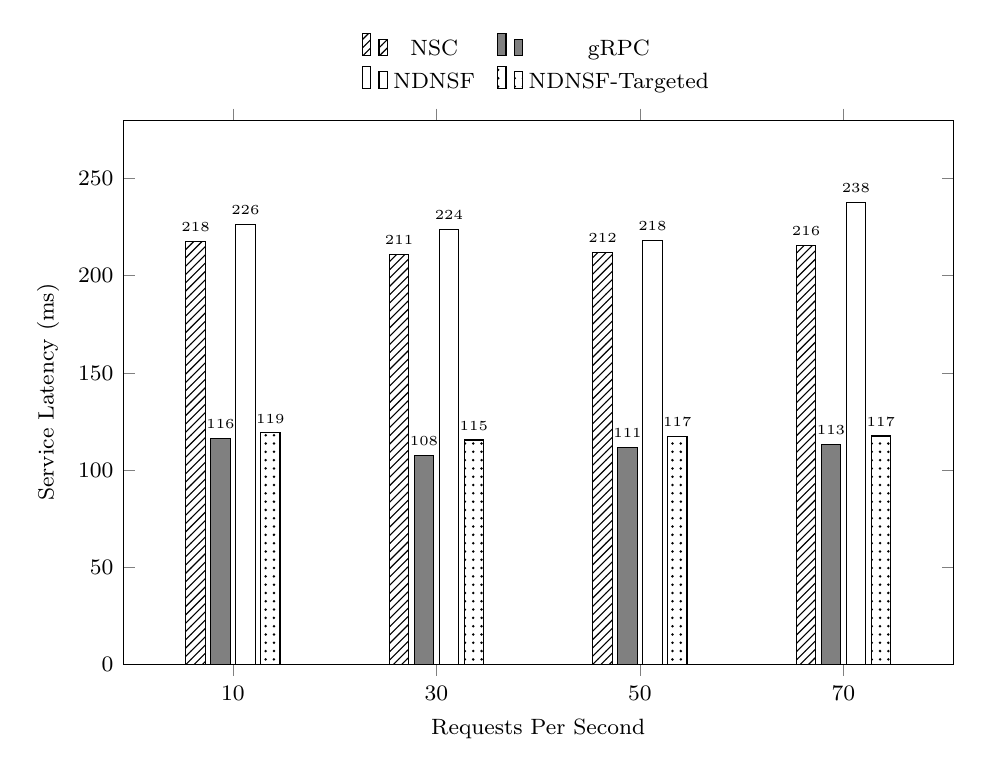
\begin{tikzpicture}
    \begin{axis}[
      ybar,
      ymin=0,
      ymax=280,
      xlabel={Requests Per Second},
      ylabel={Service Latency (ms)},
      symbolic x coords={10,30,50,70},
      xtick=data,
      ytick={0,50,100,150,200,250},
      label style={font=\footnotesize},
      tick label style={font=\footnotesize},
      nodes near coords,
      nodes near coords style={font=\tiny,
        /pgf/number format/fixed, /pgf/number format/precision=0},
      nodes near coords align={vertical},
      legend style={
        at={(0.5,1.03)},
        anchor=south,
        legend columns=2,
        draw=none,
        font=\footnotesize,
        /tikz/every even column/.append style={column sep=6pt}
      },
      bar width=7pt,
      height=0.70\columnwidth,
      width=\columnwidth,
      enlarge x limits={0.18},
      ]
      \addplot[pattern=north east lines,pattern color=black]
        coordinates {(10,217.840) (30,210.937) (50,212.190) (70,215.500)};
      \addplot[fill=gray]
        coordinates {(10,116.204) (30,107.600) (50,111.480) (70,113.300)};
      \addplot[fill=white]
        coordinates {(10,226.449) (30,223.768) (50,218.264) (70,237.604)};
      \addplot[pattern=dots,pattern color=black]
        coordinates {(10,119.092) (30,115.440) (50,117.359) (70,117.489)};
      \legend{NSC,gRPC,NDNSF,NDNSF-Targeted}
    \end{axis}
  \end{tikzpicture}
  \caption{Average Service Latency in Wired Network (Link Loss=0\%); this experimental data was collected between two nodes: Memphis and UCLA.}
  \label{fig:latency_0.00}
  \vspace{-3mm}
\end{figure}

In the no-loss comparison, Memphis and UCLA act as the service user and provider, respectively. NDNSF, NDNSF-Targeted, NSC and gRPC use the same rates of 10, 30, 50 and 70 requests per second (RPS), with a 64~B echo workload and 5\,ms service delay. A timer submits requests without waiting for earlier calls to finish. Each measurement lasts 60\,s after a 10\,s warmup; the request deadline is 5\,s. NDNSF users and providers use ECDSA runtime signatures and separate RSA keys for NAC-ABE credential delivery, with fixed-root certificate validation and a 4096~B publication-embedding threshold. NSC validates signed packets against pinned ECDSA keys, and gRPC uses mutual TLS.

Figure~\ref{fig:latency_0.00} shows that NDNSF's four-step invocation has roughly twice the mean latency of two-step targeted invocation at 10--70 RPS: 218--238\,ms versus 115--119\,ms. During measurement, all targeted calls use the Request--Response path. NDNSF has higher mean latency than NSC, while gRPC has the lowest mean latency at each rate. All four configurations submit every scheduled request and complete all measured calls within the 5\,s deadline.

\begin{figure}[!h]
  \centering
  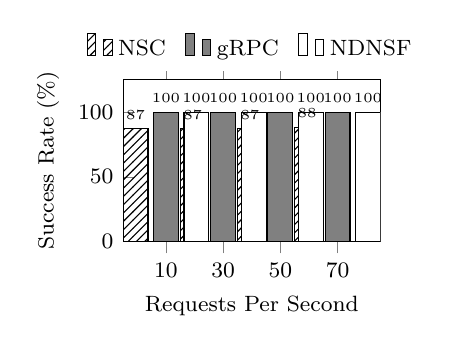
\begin{tikzpicture}
    \begin{axis}[
      ybar,
      ymin=0,
      ymax=125, % Shifted up slightly to guarantee breathing room for staggered 100s
      xlabel={Requests Per Second},
      ylabel={Success Rate (\%)},
      symbolic x coords={10,30,50,70},
      xtick=data,
      label style={font=\footnotesize},
      tick label style={font=\footnotesize},
      nodes near coords,
      % Stagger the labels so the duplicate 100 values don't collide horizontally
      nodes near coords style={
        font=\tiny,
        every node near coord/.append style={
          yshift={
            \ifnum\plotnum=1 6pt\else\ifnum\plotnum=2 1pt\else 1pt\fi\fi
          }
        }
      },
      nodes near coords align={vertical},
      legend style={
        at={(0.5,1.05)}, 
        anchor=south,
        legend columns=-1,
        draw=none,
        font=\footnotesize,
        /tikz/every even column/.append style={column sep=5pt}
      },
      bar width=9pt, % Tightened to perfectly match your 0.40\textwidth scale
      height=0.30\textwidth, 
      width=0.40\textwidth,
      enlarge x limits={0.25}, 
      ]
      \addplot[pattern=north east lines,pattern color=black] coordinates {(10,87) (30,87) (50,87) (70,88)};
      \addplot[fill=gray] coordinates {(10,100) (30,100) (50,100) (70,100)};
      \addplot[fill=white] coordinates {(10,100) (30,100) (50,100) (70,100)};
      \legend{NSC,gRPC,NDNSF}
    \end{axis}
  \end{tikzpicture}
  \caption{Success Rate in Wired Network (Link Loss=1\%, earlier implementation); this experimental data was collected between two nodes: Memphis and UCLA.}
  \label{fig:success_rate_0.01}
  %\vspace{-3mm}
\end{figure}

The separate 1\% link-loss comparison uses the earlier implementation with the 512~B publication-embedding threshold and pre-provisioned certificate configuration described above. Figure~\ref{fig:success_rate_0.01} shows that both gRPC and NDNSF maintain a 100\% success rate across all request rates. In contrast, NSC experiences 12--13\% request failures under the tested retry and timeout configuration. NDNSF therefore matches TCP-based gRPC's completion rate in that configuration.

\subsection{Reliability Under Intermittent Provider Failures}
\label{sec:intermittent-provider-failures}

\begin{table}[t]
  \centering
  \caption{
    Service Request Success Rate (\%) under Intermittent Provider Failures in a Wired Multi-Provider Environment
    %Each provider independently enters a temporary unavailable state with the specified probability.
  }
  \label{tab:success_rate_wired_intermittent}

  \small
  \setlength{\tabcolsep}{8pt}

  \begin{tabular}{lccc}
    \toprule

    \multirow{2}{*}{System}
      & \multicolumn{3}{c}{Provider Failure Probability} \\

    \cmidrule(lr){2-4}

      & 10\%
      & 20\%
      & 30\% \\

    \midrule

    NSC
      & 83.25
      & 66.58
      & 49.92 \\

    gRPC
      & 83.35
      & 66.69
      & 65.36 \\

    \textbf{NDNSF}
      & \textbf{99.82}
      & \textbf{99.46}
      & \textbf{96.70} \\

    \bottomrule
  \end{tabular}
  \vspace{-3mm}
\end{table}

In this experiment, UCLA, WUSTL, and UIUC provide identical services to Memphis. Both gRPC and NSC bind Memphis to the UCLA provider, whereas NDNSF uses the first-responding strategy to dynamically select among multiple providers. To emulate intermittent service availability, each provider independently enters a 10-second rejection period when it is unable to serve incoming requests with probability 10\%, 20\%, or 30\% every 10 seconds. For NDNSF, unavailable providers suppress ACKs, allowing the user to select another available provider when possible.

Table~\ref{tab:success_rate_wired_intermittent} shows that NDNSF achieves higher completion rates than the fixed-provider NSC and gRPC configurations at all tested rejection probabilities. When the rejection probability is 20\%, NDNSF maintains a 99.46\% success rate, while NSC and gRPC achieve only 66.58\% and 66.69\%, respectively. Even at a 30\% rejection probability, NDNSF still achieves 96.70\% success. This improvement comes from NDNSF's one-to-many service invocation model: a request can use another available provider if selection and execution finish before timeout. In contrast, the configured gRPC and NSC clients are bound to a single provider, so requests fail whenever that provider is unavailable.

\subsection{Task-Feedback Ablation}
\label{sec:task-feedback-ablation}

To isolate task feedback from access to alternative providers, we used an internal NDNSF ablation in five paired MiniNDN blocks of 13 planned tasks each. Both arms used the same two candidates, protected Request--ACK--Selection--Response path, fixed-root validation, task-state trace, 64-byte input, simulated 5-ms handler, and modeled 2-s target-recognition deadline. In both arms, the user selected the lowest provider name among the collected valid positive ACKs. Only the Provider's participation decision differed: a current-task capacity check versus ACK-all.

Each 60\,s block schedules tasks every 4.7\,s, with at most three invocation attempts per task; an attempt is a new invocation, not a message-retrieval retry. Three 1\,Gbps links have 10\,ms one-way delay and no random loss. Both providers remain reachable. Their complementary capacity states alternate at intervals of 0.3--0.7\,s (mean 0.5\,s), with each provider constrained half the time. A constrained provider cannot accept its compute- or memory-specialty task, while the other remains eligible.

Task feedback produced 65/65 timely correct completions versus 57/65 for ACK-all (paired gain 12.3 percentage points; block-bootstrap 95\% interval 7.7--18.5). It required 65 versus 89 attempts; 32 ACK-all attempts were rejected for insufficient capacity, versus none with feedback. Neither arm had duplicate or late eligible execution. Mean per-attempt submission-to-Selection time was 83.9 versus 50.1\,ms; gross relay IP traffic was 71.9 versus 99.2\,KiB per planned task. Feedback improved completion and reduced failed attempts in these traces at about 34\,ms additional selection delay. The result does not establish the same gain for other loads or deadlines.

\subsection{Matched Multi-Provider Availability}
\label{sec:matched-provider-availability}

We next compare the full NDNSF invocation path with NSC and gRPC clients that can switch between the same two providers. The testbed uses three 1\,Gbps links with 10\,ms one-way delay and no random packet loss; the offline conditions additionally apply the scheduled disconnections. Five paired MiniNDN runs per condition use the same scheduled arrivals, provider-state trace, 64-byte input, simulated 5\,ms handler and 2\,s deadline from scheduled arrival. Each 60\,s run schedules 13 tasks at 4.7\,s intervals. The conditions are stable availability, slow or fast link disconnection, and fast online busy rejection. In the offline conditions, complementary link states leave exactly one provider reachable, with each reachable half the time. State intervals average 5\,s (slow) or 0.5\,s (fast); online busy rejection uses the fast trace to alternate which provider rejects all tasks.

NDNSF uses Request--ACK--Selection--Response; NSC and gRPC retry with another provider after a failed attempt. NDNSF permits at most three invocation attempts per task; NSC and gRPC try each provider at most once (two attempts). After a timeout with possible execution, the NDNSF client keeps the attempt open until the task deadline; it retries only when non-execution is established. NDNSF allows 250\,ms for ACK collection and sets an initial 600\,ms attempt timeout, while NSC and gRPC use 250\,ms per attempt. Their security mechanisms also differ, so this comparison does not isolate cryptographic overhead. Here, correct completion requires a timely validated result without late or duplicate eligible handler execution; all planned tasks remain in the denominator. Table~\ref{tab:matched-provider-availability} reports the results.

\begin{table}[!ht]
  \centering
  \caption{Matched multi-provider results (65 tasks per arm and condition). Latency includes a 2\,s penalty for failures; gross relay IP includes background traffic.}
  \label{tab:matched-provider-availability}
  \footnotesize
  \setlength{\tabcolsep}{2.5pt}
  \begin{tabular}{lccc}
    \toprule
    \multicolumn{4}{l}{Correct tasks/65 (mean latency, ms)} \\
    Condition & NDNSF & NSC & gRPC \\
    \midrule
    Stable & 65/65 (121.6) & 65/65 (104.6) & 65/65 (56.4) \\
    Slow offline & 63/65 (374.3) & 64/65 (255.3) & 55/65 (364.6) \\
    Fast offline & 35/65 (1124.3) & 43/65 (798.5) & 31/65 (1122.2) \\
    Fast busy & 65/65 (249.5) & 63/65 (197.7) & 65/65 (82.4) \\
    \midrule
    \multicolumn{4}{l}{Gross relay IP (KiB/task)} \\
    Condition & NDNSF & NSC & gRPC \\
    \midrule
    Stable & 73.0 & 6.4 & 41.3 \\
    Slow offline & 50.9 & 6.7 & 32.2 \\
    Fast offline & 49.8 & 5.3 & 30.1 \\
    Fast busy & 88.2 & 7.6 & 39.7 \\
    \bottomrule
  \end{tabular}
\end{table}

We assess completion from task plans, handler records and terminal states, and measure traffic from packet captures. Under slow disconnection, NDNSF completes 63/65 tasks, versus 64/65 for NSC and 55/65 for gRPC (NDNSF--gRPC paired difference 12.3 percentage points; block-bootstrap 95\% interval 7.7--18.5). Under fast disconnection, NDNSF completes 35/65 versus 43/65 and 31/65; its paired difference from NSC is $-12.3$ points (interval $-26.2$ to 1.5), without an established completion advantage. NDNSF has no observed duplicate or late eligible execution. NSC and gRPC each have one duplicate execution under slow disconnection; gRPC has three under fast disconnection. In stable conditions, all three complete 65/65; under online busy rejection, their counts are 65/65, 63/65 and 65/65. NDNSF has higher mean latency and gross relay traffic in all four conditions. Different retry policies, per-attempt timeouts and transport paths prevent attributing these cross-system results to feedback alone.

We also compare five paired blocks with both providers reachable and task-specific capacity varying on the same fast trace: a constrained provider cannot accept its compute- or memory-specialty task, while the other provider remains eligible. Task classes follow a seed-shifted compute--compute--memory--memory cycle, while the NSC and gRPC clients rotate their default provider order across tasks. Generic gRPC health checks report reachability; NSC discovers task rejection after input delivery, while NDNSF receives it in ACK feedback. With the same 2\,s deadline, all three arms correctly complete 65/65 tasks without duplicate or late execution. NDNSF makes 71 attempts, versus 80 for NSC and 78 for gRPC, but its mean latency is 218.0\,ms versus 180.4 and 94.7\,ms, and gross relay IP is 78.6 versus 7.8 and 40.9\,KiB per planned task. All tasks finish within 521\,ms under this 64-byte, 5-ms-handler workload, leaving ample deadline slack. Thus, feedback avoids some retries here without improving deadline completion or offsetting its coordination cost.

\subsection{Solicitation Versus Coarse Service Advertisements}
\label{sec:dynamic-selection-cost}

We compare task-specific solicitation with preselection from long-term service advertisements followed by protected targeted requests. The advertisement arm queries status after a failed call; its change-driven publications model service capabilities, not an unmodified NDNSD implementation. In five paired blocks, two providers receive one synthetic task per second with a 2\,s deadline and an 80\,ms simulated handler. Both arms use the same eligibility checks and at most three attempts. The solicitation client waits until the task deadline if an unanswered attempt may have executed; the advertisement client can retry a targeted call after its attempt timeout. These are simulated resource and link conditions, not measured inference or flight workloads.

When temporary busy periods change task eligibility, both arms correctly complete 300/300 tasks; solicitation uses fewer submissions (313 versus 408) but more relay traffic (74.2 versus 56.5\,KiB per task). Mean latencies are 272.2 and 247.7\,ms, with no resolved paired latency difference. When complementary provider links alternate between reachable and unreachable, leaving one reachable at a time, solicitation completes 259/300 versus 270/300 tasks within 2\,s (paired difference $-3.7$ percentage points; 95\% interval $-5.3$ to $-1.7$). Its mean latency including the 2\,s failure penalty is lower (642.6 versus 732.3\,ms), but it uses more relay traffic (50.1 versus 42.1\,KiB per task). Solicitation has no observed duplicate or late eligible execution; one duplicate execution with advertisements is excluded from correct completion. Solicitation completes fewer tasks under these link changes. The comparison also changes invocation paths, retry behavior and advertisement visibility, so it does not isolate feedback alone.

\subsection{Reliability Under Mobility-Induced Disconnections}
\label{sec:mobility-induced-disconnections}

In the wireless experiments, the ground station acts as the user and the drones act as providers. The AP WiFi range is varied from 100\,m to 200\,m in the simulated coverage model. When a drone moves outside the coverage area, it becomes temporarily unavailable.

\begin{table}[!ht]
  \centering
  \caption{
    Service Request Success Rate (\%) in a Wireless Mobile Network with Different WiFi Ranges
  }
  \label{tab:success_rate_wifi_mobile}

  \small
  \setlength{\tabcolsep}{9pt}

  \begin{tabular}{lccc}
    \toprule

    \multirow{2}{*}{System}
      & \multicolumn{3}{c}{AP WiFi Range} \\

    \cmidrule(lr){2-4}

      & 100\,m
      & 150\,m
      & 200\,m \\

    \midrule

    NSC
      & 45.42
      & 68.75
      & 88.33 \\

    gRPC
      & 45.23
      & 68.05
      & 87.14 \\

    \textbf{NDNSF}
      & \textbf{96.25}
      & \textbf{100.00}
      & \textbf{100.00} \\

    \bottomrule
  \end{tabular}
\end{table}

Table~\ref{tab:success_rate_wifi_mobile} shows that NDNSF achieves higher success rates than the fixed-provider NSC and gRPC configurations under the tested mobility-induced disconnections. With a 100\,m WiFi range, NDNSF achieves a 96.25\% success rate, compared to 45.42\% for NSC and 45.23\% for gRPC. As the WiFi range increases, the success rates of all systems improve, with NDNSF having the highest reported rates in these configurations, reaching 100\% at both 150\,m and 200\,m.

This advantage stems from NDNSF's one-to-many service model. The ground station can dynamically select among multiple drones, allowing requests to use another reachable drone before timeout. In contrast, the configured gRPC and NSC clients bind the ground station to a single drone, making them more vulnerable to mobility-induced disconnections.


\subsection{ACK Strategy Evaluation}
\label{sec:selective-ack}

This experiment evaluates NDNSF's Selective ACK mechanism in a multi-provider environment. Memphis acts as the service user with a request rate of 50~RPS, while CSU, UCLA, and WUSTL provide identical services. CSU is the closest provider but is intentionally overloaded: although it continues receiving requests, it delays responses by 30~seconds. Since the request timeout is 5~seconds, requests handled by CSU are expected to fail.  We compare two ACK mechanisms. Under \emph{ACK-all}, every provider always returns an ACK, even when they cannot complete requests before timeout. Under \emph{Selective ACK}, providers suppress ACKs when overloaded, preventing themselves from being selected.

Table~\ref{tab:selective-ack} shows that ACK-all performs poorly because the first-responding strategy selects CSU for 2209 out of 2250 requests, all of which fail to return a response before the timeout, resulting in only a 1.82\% success rate. In contrast, Selective ACK prevents CSU from being selected while overloaded, allowing requests to be handled by UCLA and WUSTL and achieving a 100\% success rate. Under this forced-overload configuration, suppressing CSU's ACK prevents the first-responding strategy from choosing it.

\begin{table}[]
  \centering
  \caption{Impact of ACK Strategy When the Nearest Provider is Overloaded}
  \label{tab:selective-ack}
  \setlength{\tabcolsep}{4pt}

  \begin{tabular}{l r r r}
    \toprule
    Mechanism &
    Success &
    Selection Distribution \\
    &
    Rate &
    CSU/UCLA/WUSTL \\
    \midrule
    ACK-all       & 1.82\% & 2209/34/7 \\
    Selective ACK  & 100.00\% & 0/1723/527 \\
    \bottomrule
  \end{tabular}
  \vspace{-3mm}
\end{table}

\subsection{Provider-Selection Strategy Evaluation}
\label{sec:custom-selection}

This experiment evaluates NDNSF's customizable provider-selection mechanism. Memphis acts as the service user, while UIUC, UCLA, and WUSTL provide the same service. To create heterogeneous provider conditions, UIUC, the closest provider, is configured with the slowest service-processing delay (100\,ms), while UCLA and WUSTL use delays of 20\,ms and 5\,ms, respectively. Each provider returns ACKs carrying metadata containing current queue size. We compare two provider-selection strategies. \emph{First-Responding} selects the first provider returning a valid ACK, minimizing ACK waiting time but favoring nearby providers even when they have slower service execution. In contrast, \emph{Shortest-Queue-First}  selects the provider with the smallest reported queue.

\begin{figure}[!hb]
  \centering
  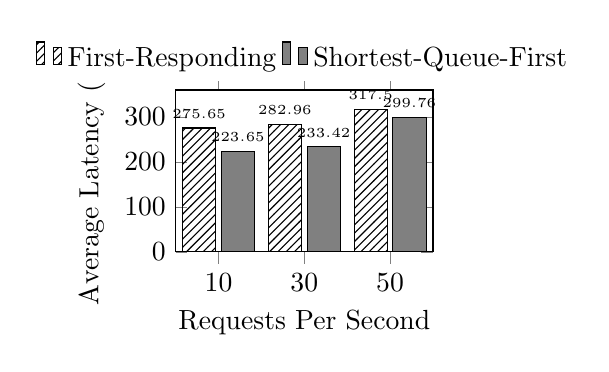
\begin{tikzpicture}
    \begin{axis}[
      ybar,
      ymin=0,
      ymax=360,
      xlabel={Requests Per Second},
      ylabel={Average Latency (ms)},
      symbolic x coords={10,30,50},
      xtick=data,
      nodes near coords,
      nodes near coords align={vertical},
      every node near coord/.append style={font=\tiny},
      legend style={at={(0.5,1.05)},
        anchor=south,legend columns=-1,draw=none},
      bar width=12pt,
      height=0.30\textwidth,
      width=0.40\textwidth,
      enlarge x limits={0.25},
      ]
      \addplot[pattern=north east lines,pattern color=black]
        coordinates {(10,275.65) (30,282.96) (50,317.50)};
      \addplot[fill=gray]
        coordinates {(10,223.65) (30,233.42) (50,299.76)};
      \legend{First-Responding, Shortest-Queue-First}
    \end{axis}
  \end{tikzpicture}
  \caption{Average Service Latency under First-Responding and Shortest-Queue-First Provider-Selection Strategies}
  \label{fig:custom-selection-avg-latency}
\end{figure}

Figure~\ref{fig:custom-selection-avg-latency} shows lower mean latency with Shortest-Queue-First at each tested rate; at 10~RPS, it is 223.65\,ms versus 275.65\,ms with First-Responding. In this configuration, using queue information offsets the additional ACK-collection delay.

\subsection{Real-World Experiments}

In the real-world experiments, the Odroid C4 acts as the service user, while the laptop and PC act as service providers. To evaluate robustness under intermittent service availability, the laptop is unavailable during the first half of the experiment, while the PC is unavailable during the middle half, leaving both providers simultaneously available only during the last quarter of the run. For gRPC and NSC, the Odroid C4 is bound to the laptop provider. In contrast, NDNSF allows both the laptop and PC to provide service to the Odroid C4.

\begin{table}[!ht]
  \centering
  \caption{Service Availability in Real-World Experiments}
  \label{tab:real_machine_availability}

  \small
  \setlength{\tabcolsep}{9pt}

  \begin{tabular}{lcc}
    \toprule
    System & 10 RPS & 30 RPS \\
    \midrule
    NSC   & 52.67\% & 51.78\% \\
    gRPC  & 49.33\% & 47.06\% \\
    \textbf{NDNSF} & \textbf{74.62\%} & \textbf{73.73\%} \\
    \bottomrule
  \end{tabular}
  \vspace{-3mm}
\end{table}

Table~\ref{tab:real_machine_availability} reports the resulting service request success rates. Because gRPC and NSC rely on a fixed provider, their success rates remain near 50\%, matching the provider availability period. NDNSF can select a reachable provider when one is available, achieving a success rate close to the expected 75\% service-availability window. This comparison supports the benefit of access to alternative providers, but does not isolate task-specific feedback.


\section{RELATED WORK}
Existing service invocation, publication, and access-control mechanisms provide the basis for NDNSF's candidate discovery and permission management.

RICE~\cite{krol2018rice} studies remote method invocation in ICN, including an invocation handshake and parameter/result handling. NDNSF builds on these established ideas for invocation and protected parameter exchange.

DNMP~\cite{nichols2019dnmp} publishes measurement commands through Sync and collects replies. VerSec relates allowed command components to role signing keys. The schema determines which roles may issue commands with particular targets and parameters.

NDNSF instead uses service-attribute encryption to restrict descriptor readers and aggregates permissions in DKEYs. Adding encryption to a DNMP-style design would also protect command content, with additional key-distribution costs.

NSC~\cite{meirovitch2021nsc} requires a signed initial invocation Interest, uses application-defined trust schemas, and describes encrypted input/result retrieval with NAC support. Its report also discusses retry behavior for long-running computation.

NDNSF explicitly collects candidate feedback before selection. This differs from the basic NSC invocation sequence, but applications can extend an invocation system with discovery or negotiation; their complete costs must be compared.

NDNSD~\cite{dulal2022ndnsd} supports service advertisement discovery and optional NAC-ABE protection of service information. NDNSF can use these advertisements for provider preselection, while its Request--ACK exchange obtains participation feedback for a particular task.

NAC~\cite{zhang2018nac} automates named-data access-key distribution and analyzes ABE-based aggregation. Enhanced NAC-ABE supplies KP-ABE, policy-bearing DKEYs, validation support, and key segmentation~\cite{dulal2023nac-abe}.

NDNSF applies these capabilities to service descriptors and invocation permissions. The reduction in credential objects follows from ABE permission aggregation. Section~\ref{sec:credential-cost} examines this benefit and its key-distribution and update costs.

Trust schemas can encode general rules rather than one rule per entity or service~\cite{yu2015trust}. Other designs can also reuse identity credentials and general trust rules. NDNSF keeps service-permission lists in ABE policies rather than baseline trust rules; this does not establish lower rule-management or validation costs than every alternative.


\section{CONCLUSION AND FUTURE WORK}
NDNSF provides a general framework for building service-oriented distributed applications, supporting diverse service types and adapting to varied requirements. It enables fine-grained control over which providers can offer a service and which users can invoke it. Through protected Request--ACK exchanges and user-side selection, a user can invoke the same service across multiple providers. In the single-provider wired loss experiment, NDNSF achieves higher completion rates than NSC and rates comparable to gRPC. In the intermittent-availability comparisons, it achieves higher completion rates than fixed-provider configurations. A controlled ablation shows that task-specific feedback improves deadline completion under changing provider capacity. Against baselines with the same preconfigured candidates and the ability to retry another provider, NDNSF shows no consistent completion advantage and has higher invocation latency and traffic. The costs of obtaining and updating candidate lists are outside that comparison. Under one ABE authority, NAC-ABE aggregates an entity's service permissions in one decryption key. At larger permission counts, this reduces initial distribution and key-rotation costs relative to separate ABE keys for each permission. In the evaluated scheme, granting a permission updates one entity's decryption key, whereas revoking all of that entity's service permissions requires key rotation and redistribution to the remaining authorized entities.

Future work will extend NDNSF's APIs to coordinate multiple providers in collaboratively executing complex tasks. We will further develop and evaluate UAV and distributed AI inference applications built on NDNSF.


%LW: remove for submission for anonymity
%\section*{Disclaimer}
%This material is based upon work supported by the National Science Foundation while Lan Wang was serving at the National Science Foundation. Any opinion, findings, and conclusions or recommendations expressed in this material are those of the author(s) and do not necessarily reflect the views of the National Science Foundation.


% An example of a floating figure using the graphicx package.
% Note that \label must occur AFTER (or within) \caption.
% For figures, \caption should occur after the \includegraphics.
% Note that IEEEtran v1.7 and later has special internal code that
% is designed to preserve the operation of \label within \caption
% even when the captionsoff option is in effect. However, because
% of issues like this, it may be the safest practice to put all your
% \label just after \caption rather than within \caption{}.
%
% Reminder: the "draftcls" or "draftclsnofoot", not "draft", class
% option should be used if it is desired that the figures are to be
% displayed while in draft mode.
%
%\begin{figure}[!t]
%\centering
%\includegraphics[width=2.5in]{myfigure}
% where an .eps filename suffix will be assumed under latex, 
% and a .pdf suffix will be assumed for pdflatex; or what has been declared
% via \DeclareGraphicsExtensions.
%\caption{Simulation results for the network.}
%\label{fig_sim}
%\end{figure}

% Note that the IEEE typically puts floats only at the top, even when this
% results in a large percentage of a column being occupied by floats.


% An example of a double column floating figure using two subfigures.
% (The subfig.sty package must be loaded for this to work.)
% The subfigure \label commands are set within each subfloat command,
% and the \label for the overall figure must come after \caption.
% \hfil is used as a separator to get equal spacing.
% Watch out that the combined width of all the subfigures on a 
% line do not exceed the text width or a line break will occur.
%
%\begin{figure*}[!t]
%\centering
%\subfloat[Case I]{\includegraphics[width=2.5in]{box}%
%\label{fig_first_case}}
%\hfil
%\subfloat[Case II]{\includegraphics[width=2.5in]{box}%
%\label{fig_second_case}}
%\caption{Simulation results for the network.}
%\label{fig_sim}
%\end{figure*}
%
% Note that often IEEE papers with subfigures do not employ subfigure
% captions (using the optional argument to \subfloat[]), but instead will
% reference/describe all of them (a), (b), etc., within the main caption.
% Be aware that for subfig.sty to generate the (a), (b), etc., subfigure
% labels, the optional argument to \subfloat must be present. If a
% subcaption is not desired, just leave its contents blank,
% e.g., \subfloat[].


% An example of a floating table. Note that, for IEEE style tables, the
% \caption command should come BEFORE the table and, given that table
% captions serve much like titles, are usually capitalized except for words
% such as a, an, and, as, at, but, by, for, in, nor, of, on, or, the, to
% and up, which are usually not capitalized unless they are the first or
% last word of the caption. Table text will default to \footnotesize as
% the IEEE normally uses this smaller font for tables.
% The \label must come after \caption as always.
%
%\begin{table}[!t]
%% increase table row spacing, adjust to taste
%\renewcommand{\arraystretch}{1.3}
% if using array.sty, it might be a good idea to tweak the value of
% \extrarowheight as needed to properly center the text within the cells
%\caption{An Example of a Table}
%\label{table_example}
%\centering
%% Some packages, such as MDW tools, offer better commands for making tables
%% than the plain LaTeX2e tabular which is used here.
%\begin{tabular}{|c||c|}
%\hline
%One & Two\\
%\hline
%Three & Four\\
%\hline
%\end{tabular}
%\end{table}


% Note that the IEEE does not put floats in the very first column
% - or typically anywhere on the first page for that matter. Also,
% in-text middle ("here") positioning is typically not used, but it
% is allowed and encouraged for Computer Society conferences (but
% not Computer Society journals). Most IEEE journals/conferences use
% top floats exclusively. 
% Note that, LaTeX2e, unlike IEEE journals/conferences, places
% footnotes above bottom floats. This can be corrected via the
% \fnbelowfloat command of the stfloats package.









% if have a single appendix:
%\appendix[Proof of the Zonklar Equations]
% or
%\appendix  % for no appendix heading
% do not use \section anymore after \appendix, only \section*
% is possibly needed

% use appendices with more than one appendix
% then use \section to start each appendix
% you must declare a \section before using any
% \subsection or using \label (\appendices by itself
% starts a section numbered zero.)
%










% Can use something like this to put references on a page
% by themselves when using endfloat and the captionsoff option.
\ifCLASSOPTIONcaptionsoff
  \newpage
\fi



% trigger a \newpage just before the given reference
% number - used to balance the columns on the last page
% adjust value as needed - may need to be readjusted if
% the document is modified later
%\IEEEtriggeratref{8}
% The "triggered" command can be changed if desired:
%\IEEEtriggercmd{\enlargethispage{-5in}}

% references section

% can use a bibliography generated by BibTeX as a .bbl file
% BibTeX documentation can be easily obtained at:
% http://mirror.ctan.org/biblio/bibtex/contrib/doc/
% The IEEEtran BibTeX style support page is at:
% http://www.michaelshell.org/tex/ieeetran/bibtex/
%\bibliographystyle{IEEEtran}
% argument is your BibTeX string definitions and bibliography database(s)
%\bibliography{IEEEabrv,../bib/paper}
%
% <OR> manually copy in the resultant .bbl file
% set second argument of \begin to the number of references
% (used to reserve space for the reference number labels box)


\bibliographystyle{IEEEtran}
\bibliography{sections/references}



% You can push biographies down or up by placing
% a \vfill before or after them. The appropriate
% use of \vfill depends on what kind of text is
% on the last page and whether or not the columns
% are being equalized.

%\vfill

% Can be used to pull up biographies so that the bottom of the last one
% is flush with the other column.
%\enlargethispage{-5in}



% that's all folks
\end{document}


